%!TEX root = ../../../adrien_gomar_phd.tex

\subsection{Analysis of the convergence}
\label{sub:dream_hs_steady_conv}

The convergence of the simulation is obtained 
after 500 iterations for both
the residuals and the similarity coefficients 
(Figure~\ref{fig:dream_HS_convergence_roe2}). More than
five orders of magnitude are obtained for the residuals and
the similarity coefficients are stabilized starting below
$1,000$ iterations. According to \citet{Casey2000},
this means that the steady simulation is converged.
\begin{figure}[htp]
  \centering
  \subfigure[residuals]{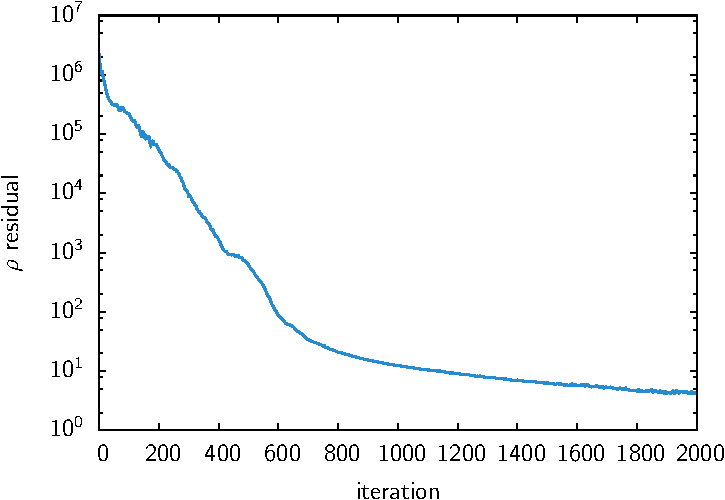
\includegraphics[width=.35\textwidth]{DREAM_HS_RESIDUALS_PPT.pdf}}
  \subfigure[thrust coefficient]{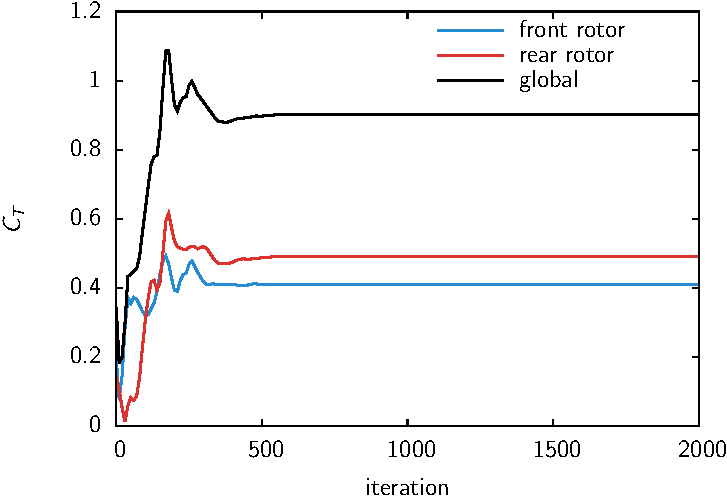
\includegraphics[width=.35\textwidth]{DREAM_HS_FORCES_CT_PPT.pdf}}
  \subfigure[power coefficient]{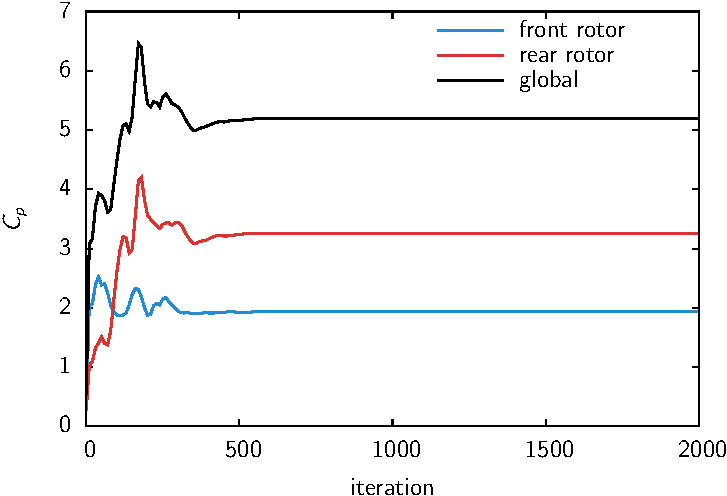
\includegraphics[width=.35\textwidth]{DREAM_HS_FORCES_CP_PPT.pdf}}
  \subfigure[efficiency]{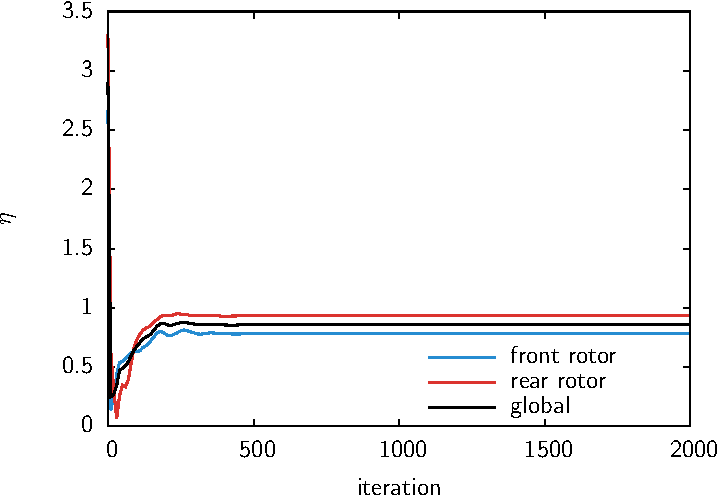
\includegraphics[width=.35\textwidth]{DREAM_HS_FORCES_ETA_PPT.pdf}}
  \caption{High-speed isolated configuration: convergence of the steady
  computation.}
  \label{fig:dream_HS_convergence_roe2}
\end{figure}

\subsection{Similarity coefficients}
\label{sub:dream_hs_sim_coeff}

The similarity coefficients are reported in 
Tab.~\ref{tab:dream_HS_sim_coeff}. 
They are representative of a cruise
propeller (see Eq.~\eqref{eq:estimation_sim_coeff}). 
Firstly, the thrust is higher
on the rear rotor than on the front rotor, even though it is
relatively well distributed. Bare in mind that the rear rotor
similarity coefficient is normalized by the front rotor diameter. Therefore, 
the thrust produced by the rear rotor is larger than the one of the front rotor, 
relatively to its diameter. 
Secondly, the power coefficient is similar for both the front and the
rear rotor. As the power coefficient represents the mechanical input
given to flow, this means that the mechanical distribution is 
well repartitioned, which is a design wish for the integrity of
the drive shaft. In fact a non-uniform power coefficient
might give an additional momentum on the drive shaft which can
deteriorates its mechanical properties.
\begin{table}[htp]
  \ra{1.3} \centering
  \begin{tabular}{ccc||ccc|ccc}
    \toprule
    \multicolumn{3}{c||}{global} & \multicolumn{3}{c|}{front} & \multicolumn{3}{c}{rear} \\
    $C_T$ & $C_P$ & $\eta$ & $C_{T_f}$ & $C_{P_f}$ & $\eta_f$ & $C_{T_r}$ & $C_{P_r}$ & $\eta_r$ \\
    \midrule
    0.902 & 3.849 & 0.858 & 0.411 & 1.926 & 0.780 & 0.491 & 1.922 & 0.935 \\
    \bottomrule
  \end{tabular}
  \caption{High-speed isolated configuration: similarity coefficients.}
  \label{tab:dream_HS_sim_coeff}
\end{table}

\subsection{Radial profiles}
\label{sub:dream_hs_radial_profiles}

Radial profiles are computed on the steady results and 
reported in Figure~\ref{fig:dream_HS_radial_profiles}.
\begin{figure}[htp]
  \centering
  \subfigure[absolute Mach number]{
    \label{fig:dream_HS_radial_profiles_ma}
    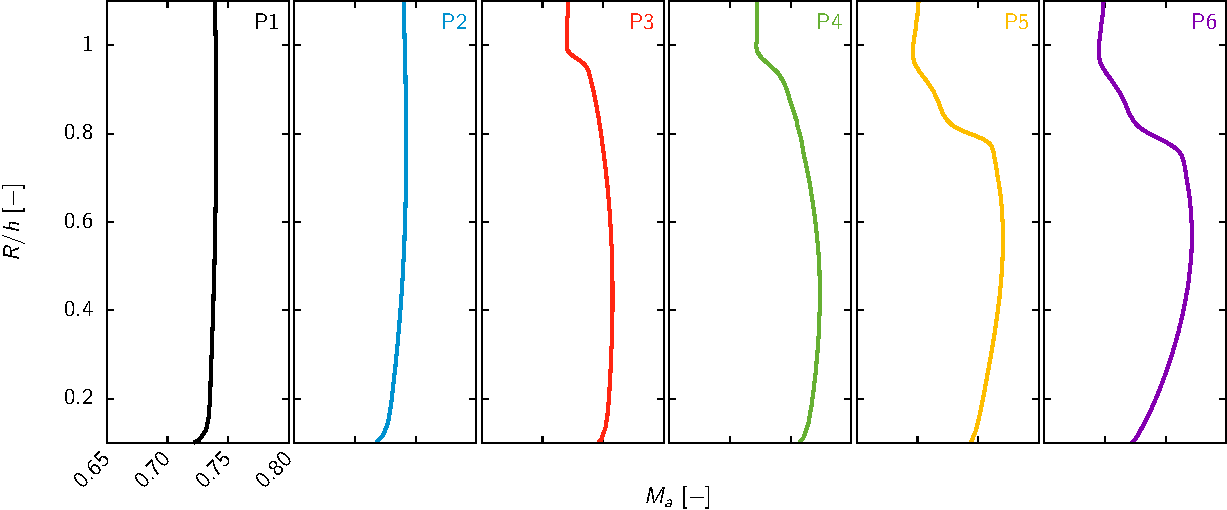
\includegraphics[width=.72\textwidth]{DREAM_HS_RANS_AZI_MEAN_PPT_macha.pdf}}
  \subfigure[absolute flow angle]{
    \label{fig:dream_HS_radial_profiles_alpha}
    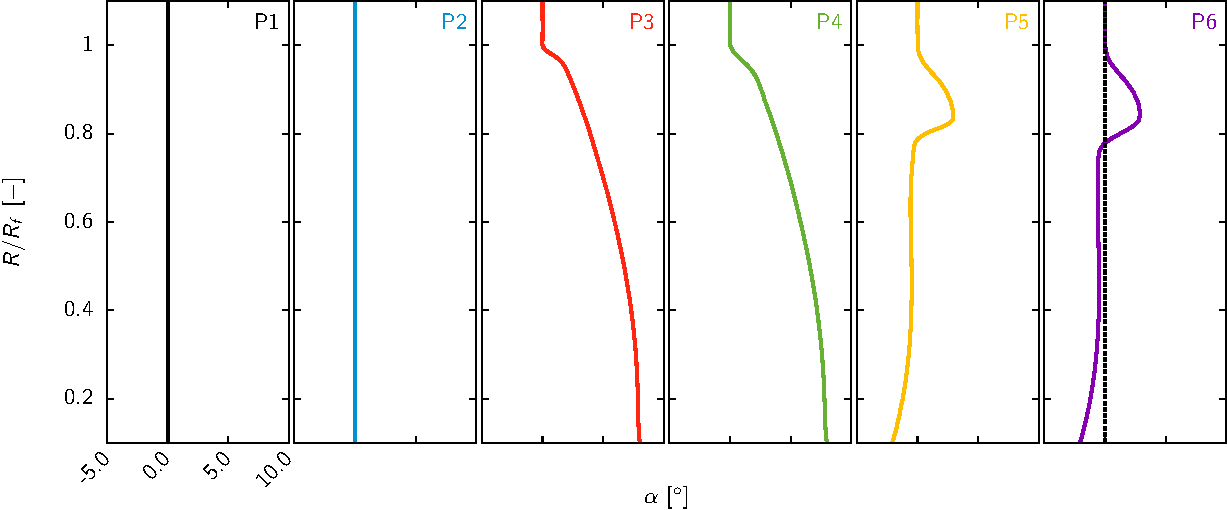
\includegraphics[width=.72\textwidth]{DREAM_HS_RANS_AZI_MEAN_PPT_alpha.pdf}}
  \caption{High-speed isolated configuration: radial profiles.}
\end{figure}
\setcounter{figure}{\value{figure}-1}
\begin{figure}[htp]
  \centering
  \setcounter{subfigure}{3}
  \subfigure[static pressure]{
    \label{fig:dream_HS_radial_profiles_ps}
    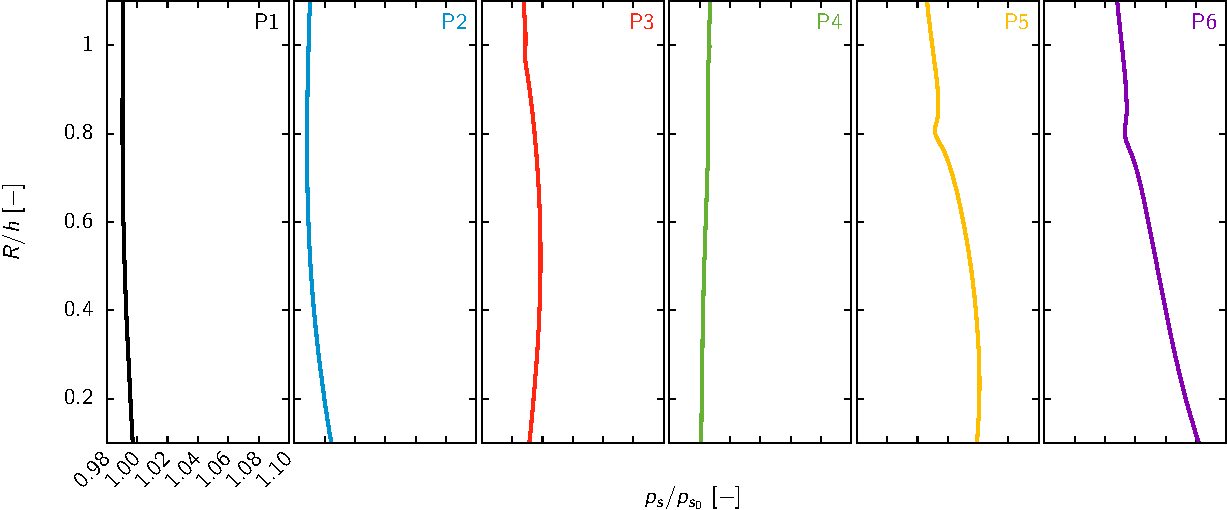
\includegraphics[width=.72\textwidth]{DREAM_HS_RANS_AZI_MEAN_PPT_ps.pdf}}
  \subfigure[stagnation temperature]{
    \label{fig:dream_HS_radial_profiles_ti}
    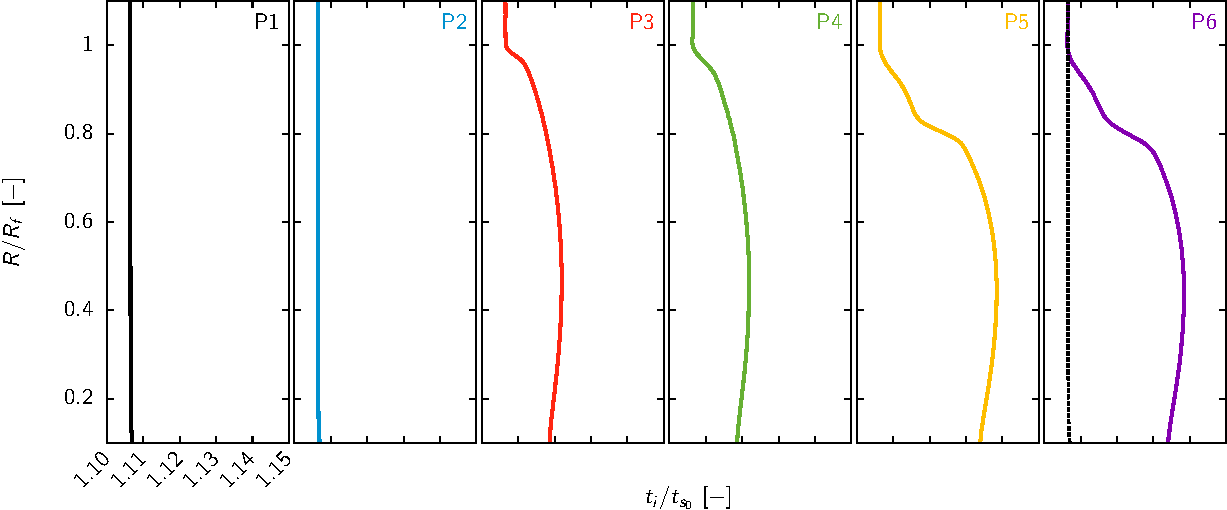
\includegraphics[width=.72\textwidth]{DREAM_HS_RANS_AZI_MEAN_PPT_ti.pdf}}
  \subfigure[stagnation pressure]{
    \label{fig:dream_HS_radial_profiles_pi}
    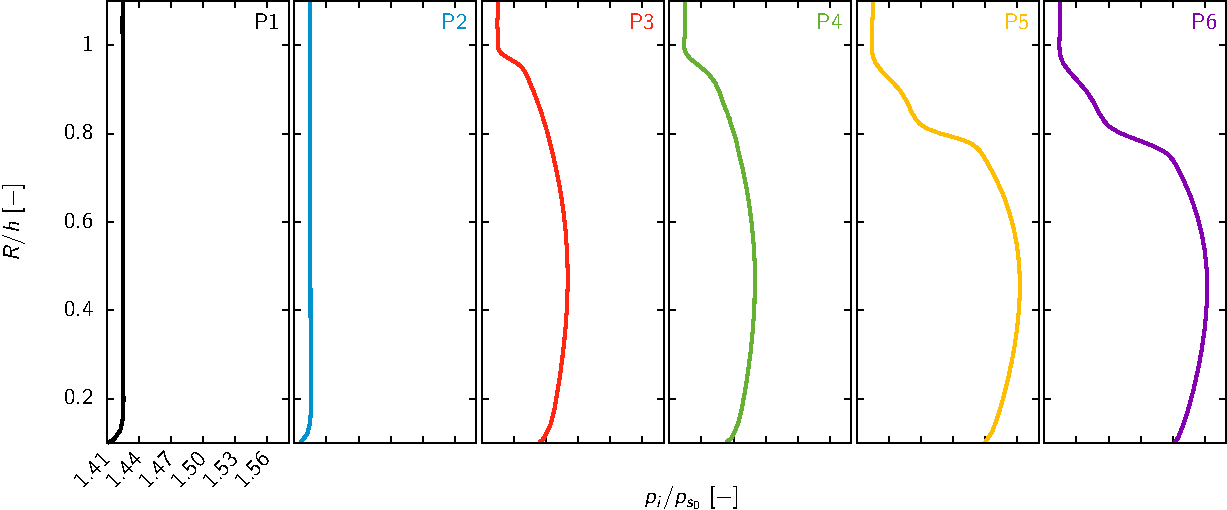
\includegraphics[width=.72\textwidth]{DREAM_HS_RANS_AZI_MEAN_PPT_pi.pdf}}
  \caption{High-speed isolated configuration: radial profiles (contd.).}
  \label{fig:dream_HS_radial_profiles}
\end{figure}

The absolute Mach number (Figure~\ref{fig:dream_HS_radial_profiles_ma}) 
increases from its inflow
value ($M_a = 0.73$) up to around $M_a=0.76$. This represents
a 4\% increase that has to be compared to the 100\% increase
for the low-speed configuration. Nevertheless, this represents
an absolute $\Delta M_a = 0.03$ increase for this high-speed
configuration where it was $\Delta M_a = 0.2$
for the low-speed configuration. The stream tube contraction
is smaller than the low-speed configuration 
as the increase in velocity remains bounded.
It seems that the front rotor tip vortices do not interact
with the rear rotor blades as the small increase near 90\%
of the span, which is attributed to the core of the vortices,
is not contracted by the stream tube.

The absolute pitch angle (Figure~\ref{fig:dream_HS_radial_profiles_alpha}) 
of the velocity highlights, again, the advantage
of using a CROR compared to a single row propeller system. In fact,
the flow is deviated by the front rotor from its axial direction
to a mean $5^\circ$ velocity vector. The rear rotor then deviates
back the flow field to make it almost purely axial with exceptions
near the hub and near the front tip vortex region ($0.75 \leq R/R_f \leq 0.95$).
This explains the efficiency of a CROR propeller system also for high-speed
inflow conditions, which is the design priority.

The static pressure (Figure~\ref{fig:dream_HS_radial_profiles_ps}) increases
by at-most 10\% which is larger than it was for the low-speed
inflow condition. These are clearly compressibility effects due
to the high inflow Mach number. As the goal of a CROR is
to create thrust through a large mass-flow, this
static pressure rise helps increasing the mass-flow.
In fact, using roughly the perfect gas state-equation,
a static pressure increase is seen as a density increase that
participates to a high mass-flow, hence the contribution to thrust.
In fact, a larger part of the energy is converted to static
pressure and not to velocity. The potential effects can be seen in the
$P2$ and $P4$ planes. In fact, the pressure decreases before
crossing a rotor blades. This is due to the acceleration of the
fluid that is done at each rotor crossing. This increase of velocity
creates a decrease in static pressure that is seen upstream the rotors.

With the stagnation temperature rise shown
in Figure~\ref{fig:dream_HS_radial_profiles_ti}, one can say that
the rotors provide energy to the fluid to create the thrust.
The stagnation pressure is shown in Figure~\ref{fig:dream_HS_radial_profiles_pi}.
At each rotor crossing it increases since both the absolute velocity and
the static pressure increase. 
Moreover, the stream tube contraction seems to be lessened
compared to the low-speed flight condition. It will have to be
confirmed by the forthcoming unsteady results.

\subsection{Flow field around the blades}
\label{sub:dream_hs_blades}

Relative Mach number contours and the pressure coefficient
$k_p$ are shown in Figure~\ref{fig:dream_HS_mach_kp} for both the
front and the rear rotors.
\begin{figure}[htp]
 \centering
 \begin{tabular}{rccc}
   & $k_p$ front rotor
   & $k_p$ rear rotor
   & relative Mach number\\
   \rotatebox{90}{\qquad\qquad 25~\%} 
   & 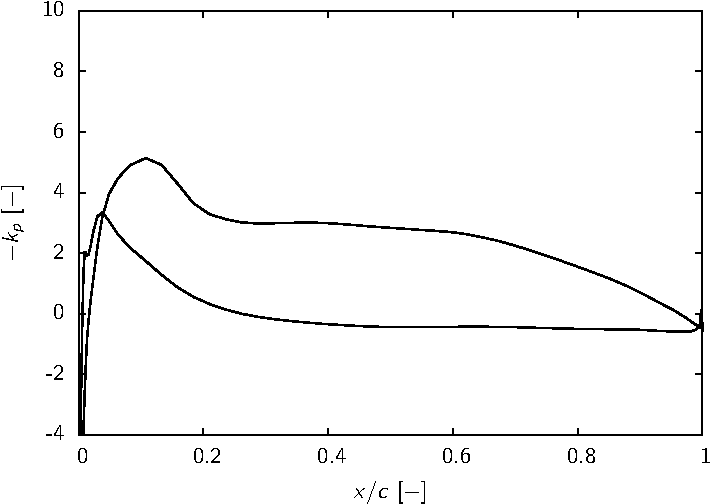
\includegraphics[width=0.28\textwidth]{DREAM_HS_KP_25_FRONT_PPT.pdf}
   & 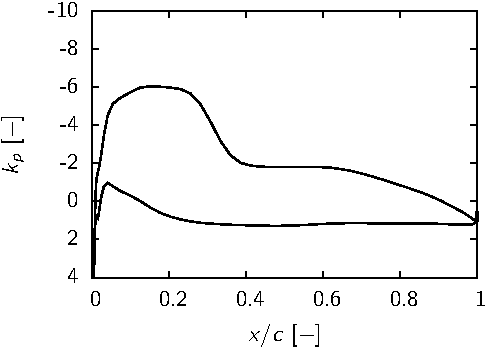
\includegraphics[width=0.28\textwidth]{DREAM_HS_KP_25_REAR_PPT.pdf}
   & 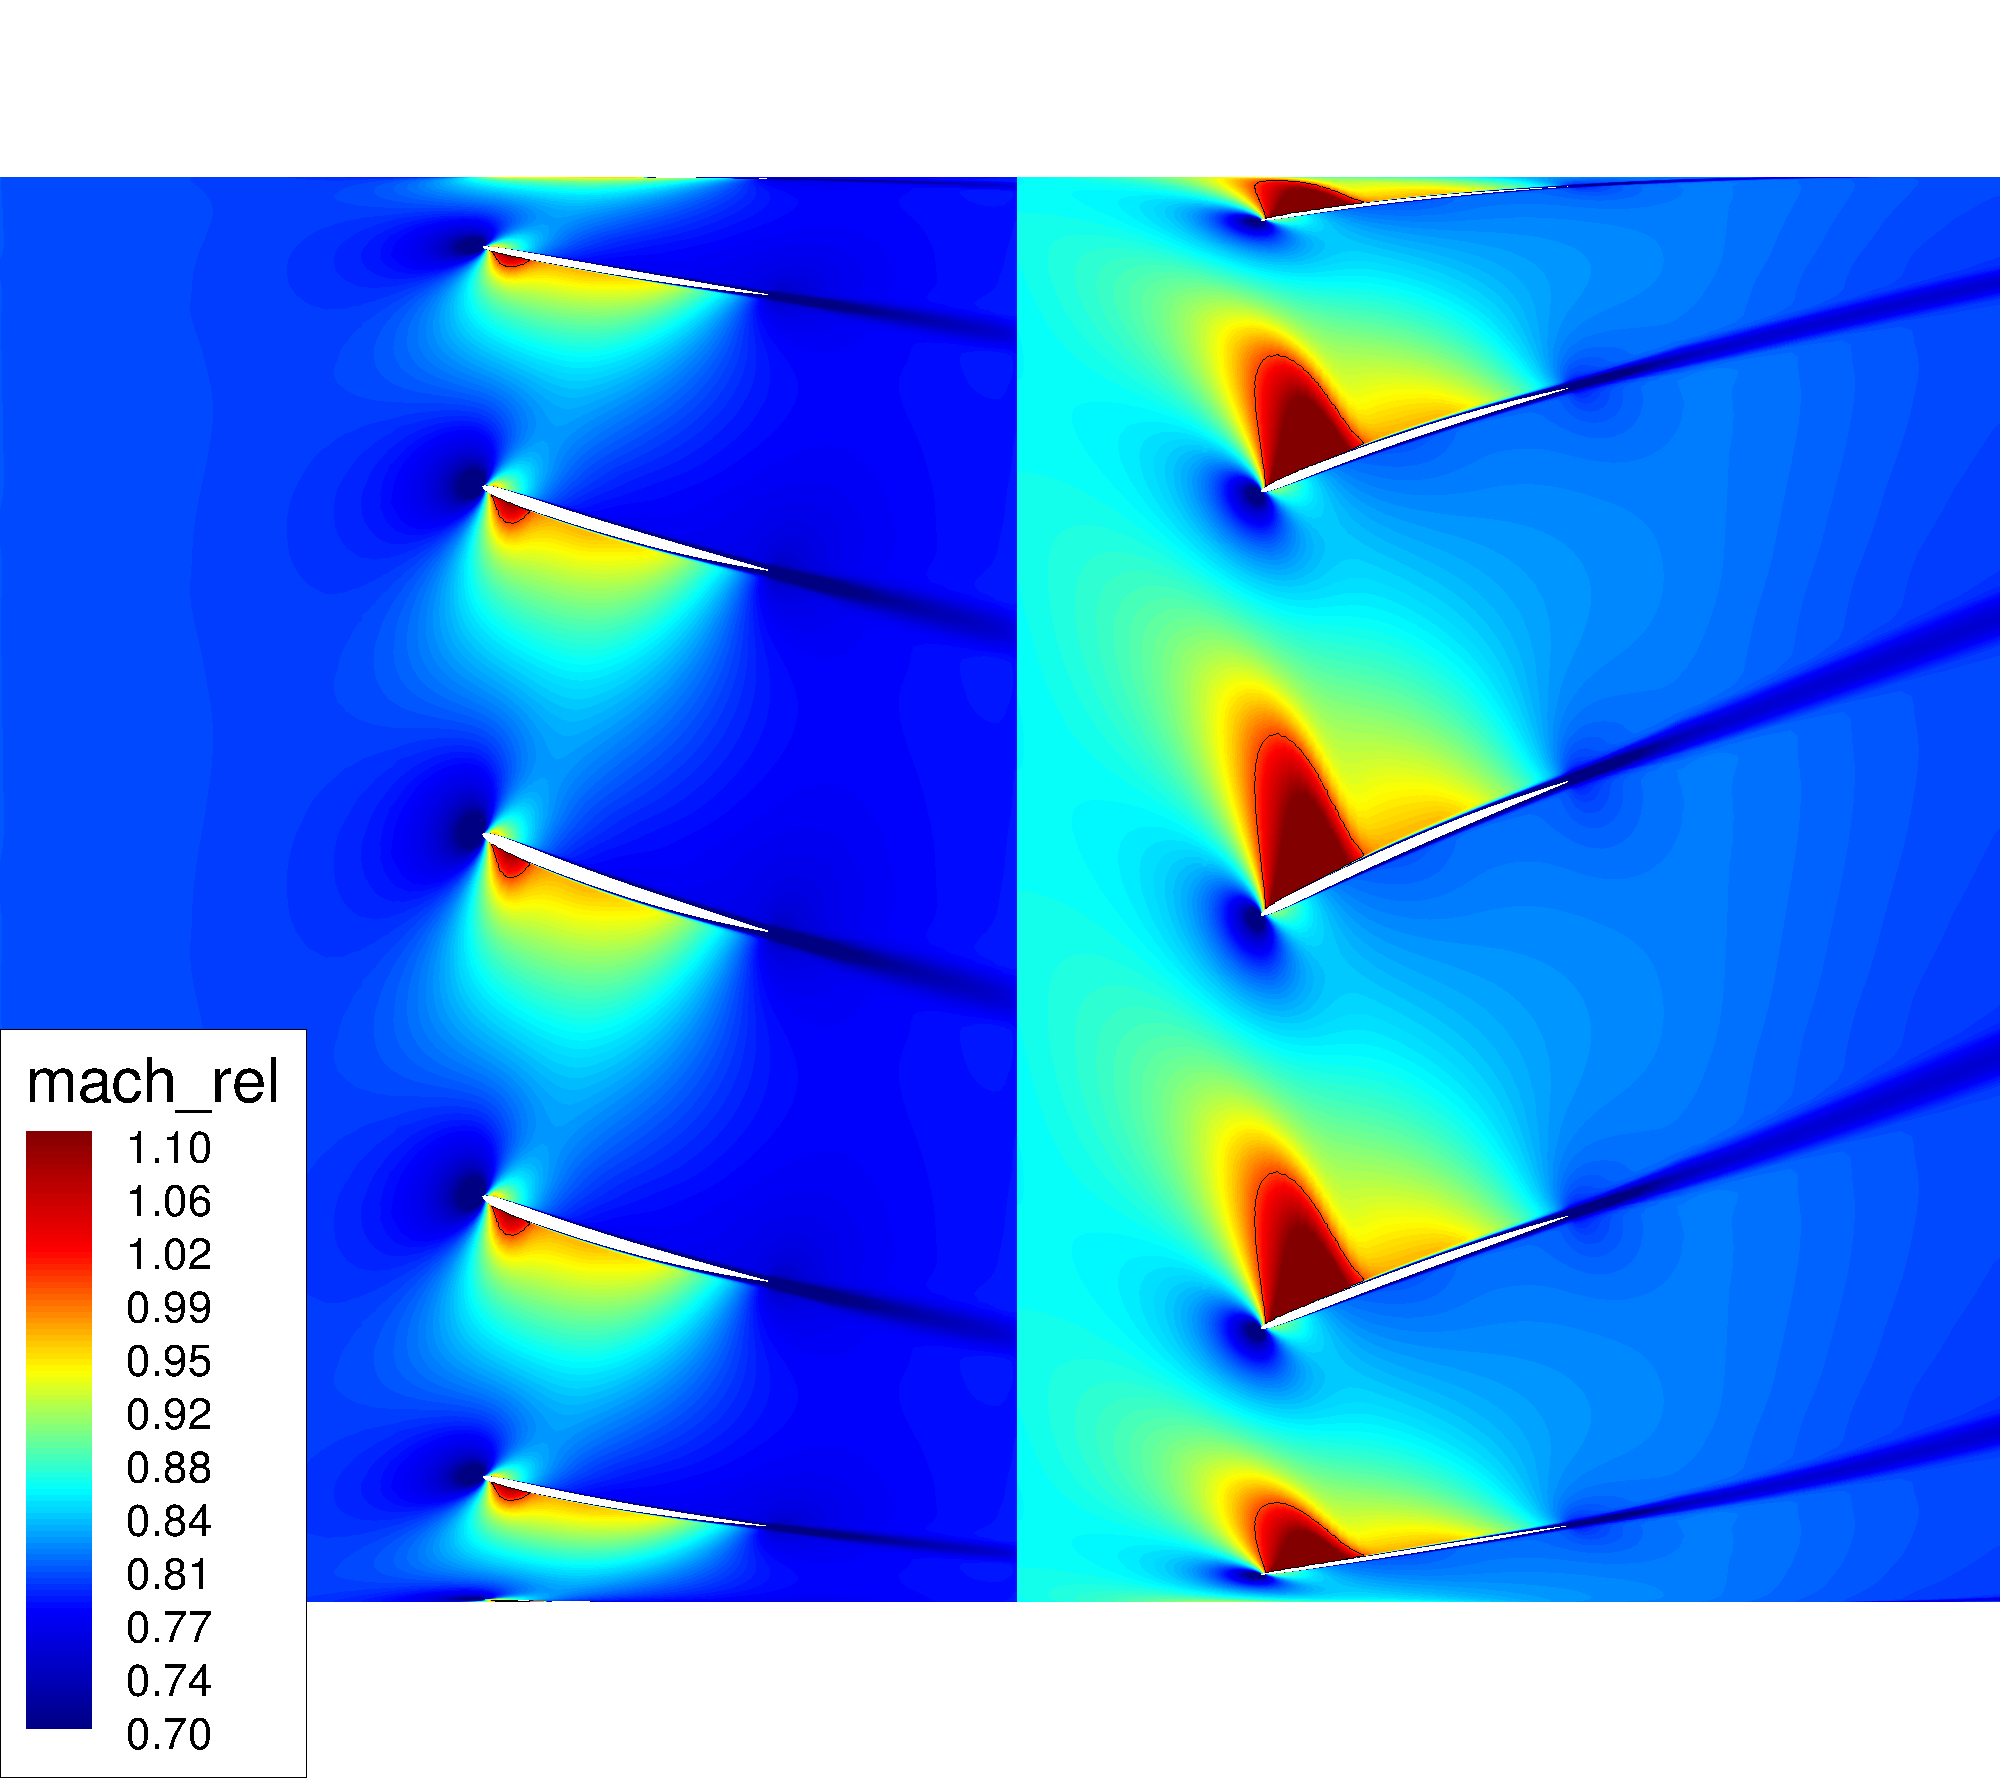
\includegraphics[width=0.28\textwidth]{DREAM_HS_RANS_roe2_sa_slice_r_25_mach_rel.png}\\
   \rotatebox{90}{\qquad\qquad 50~\%} 
   & 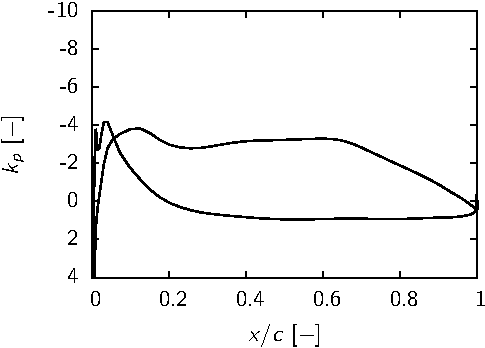
\includegraphics[width=0.28\textwidth]{DREAM_HS_KP_50_FRONT_PPT.pdf}
   & 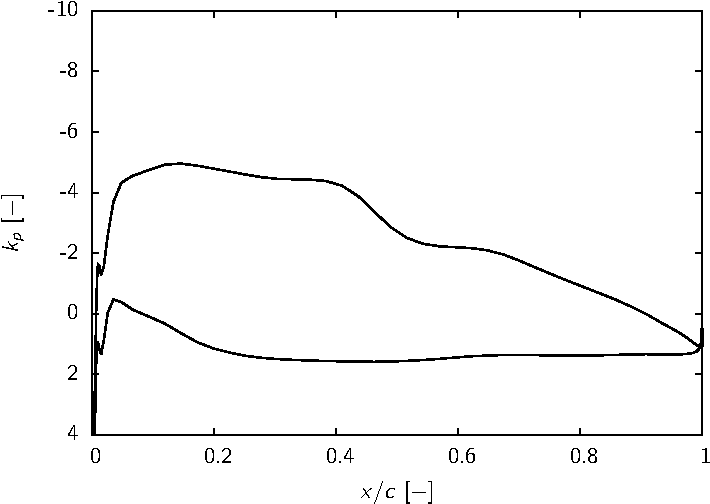
\includegraphics[width=0.28\textwidth]{DREAM_HS_KP_50_REAR_PPT.pdf}
   & 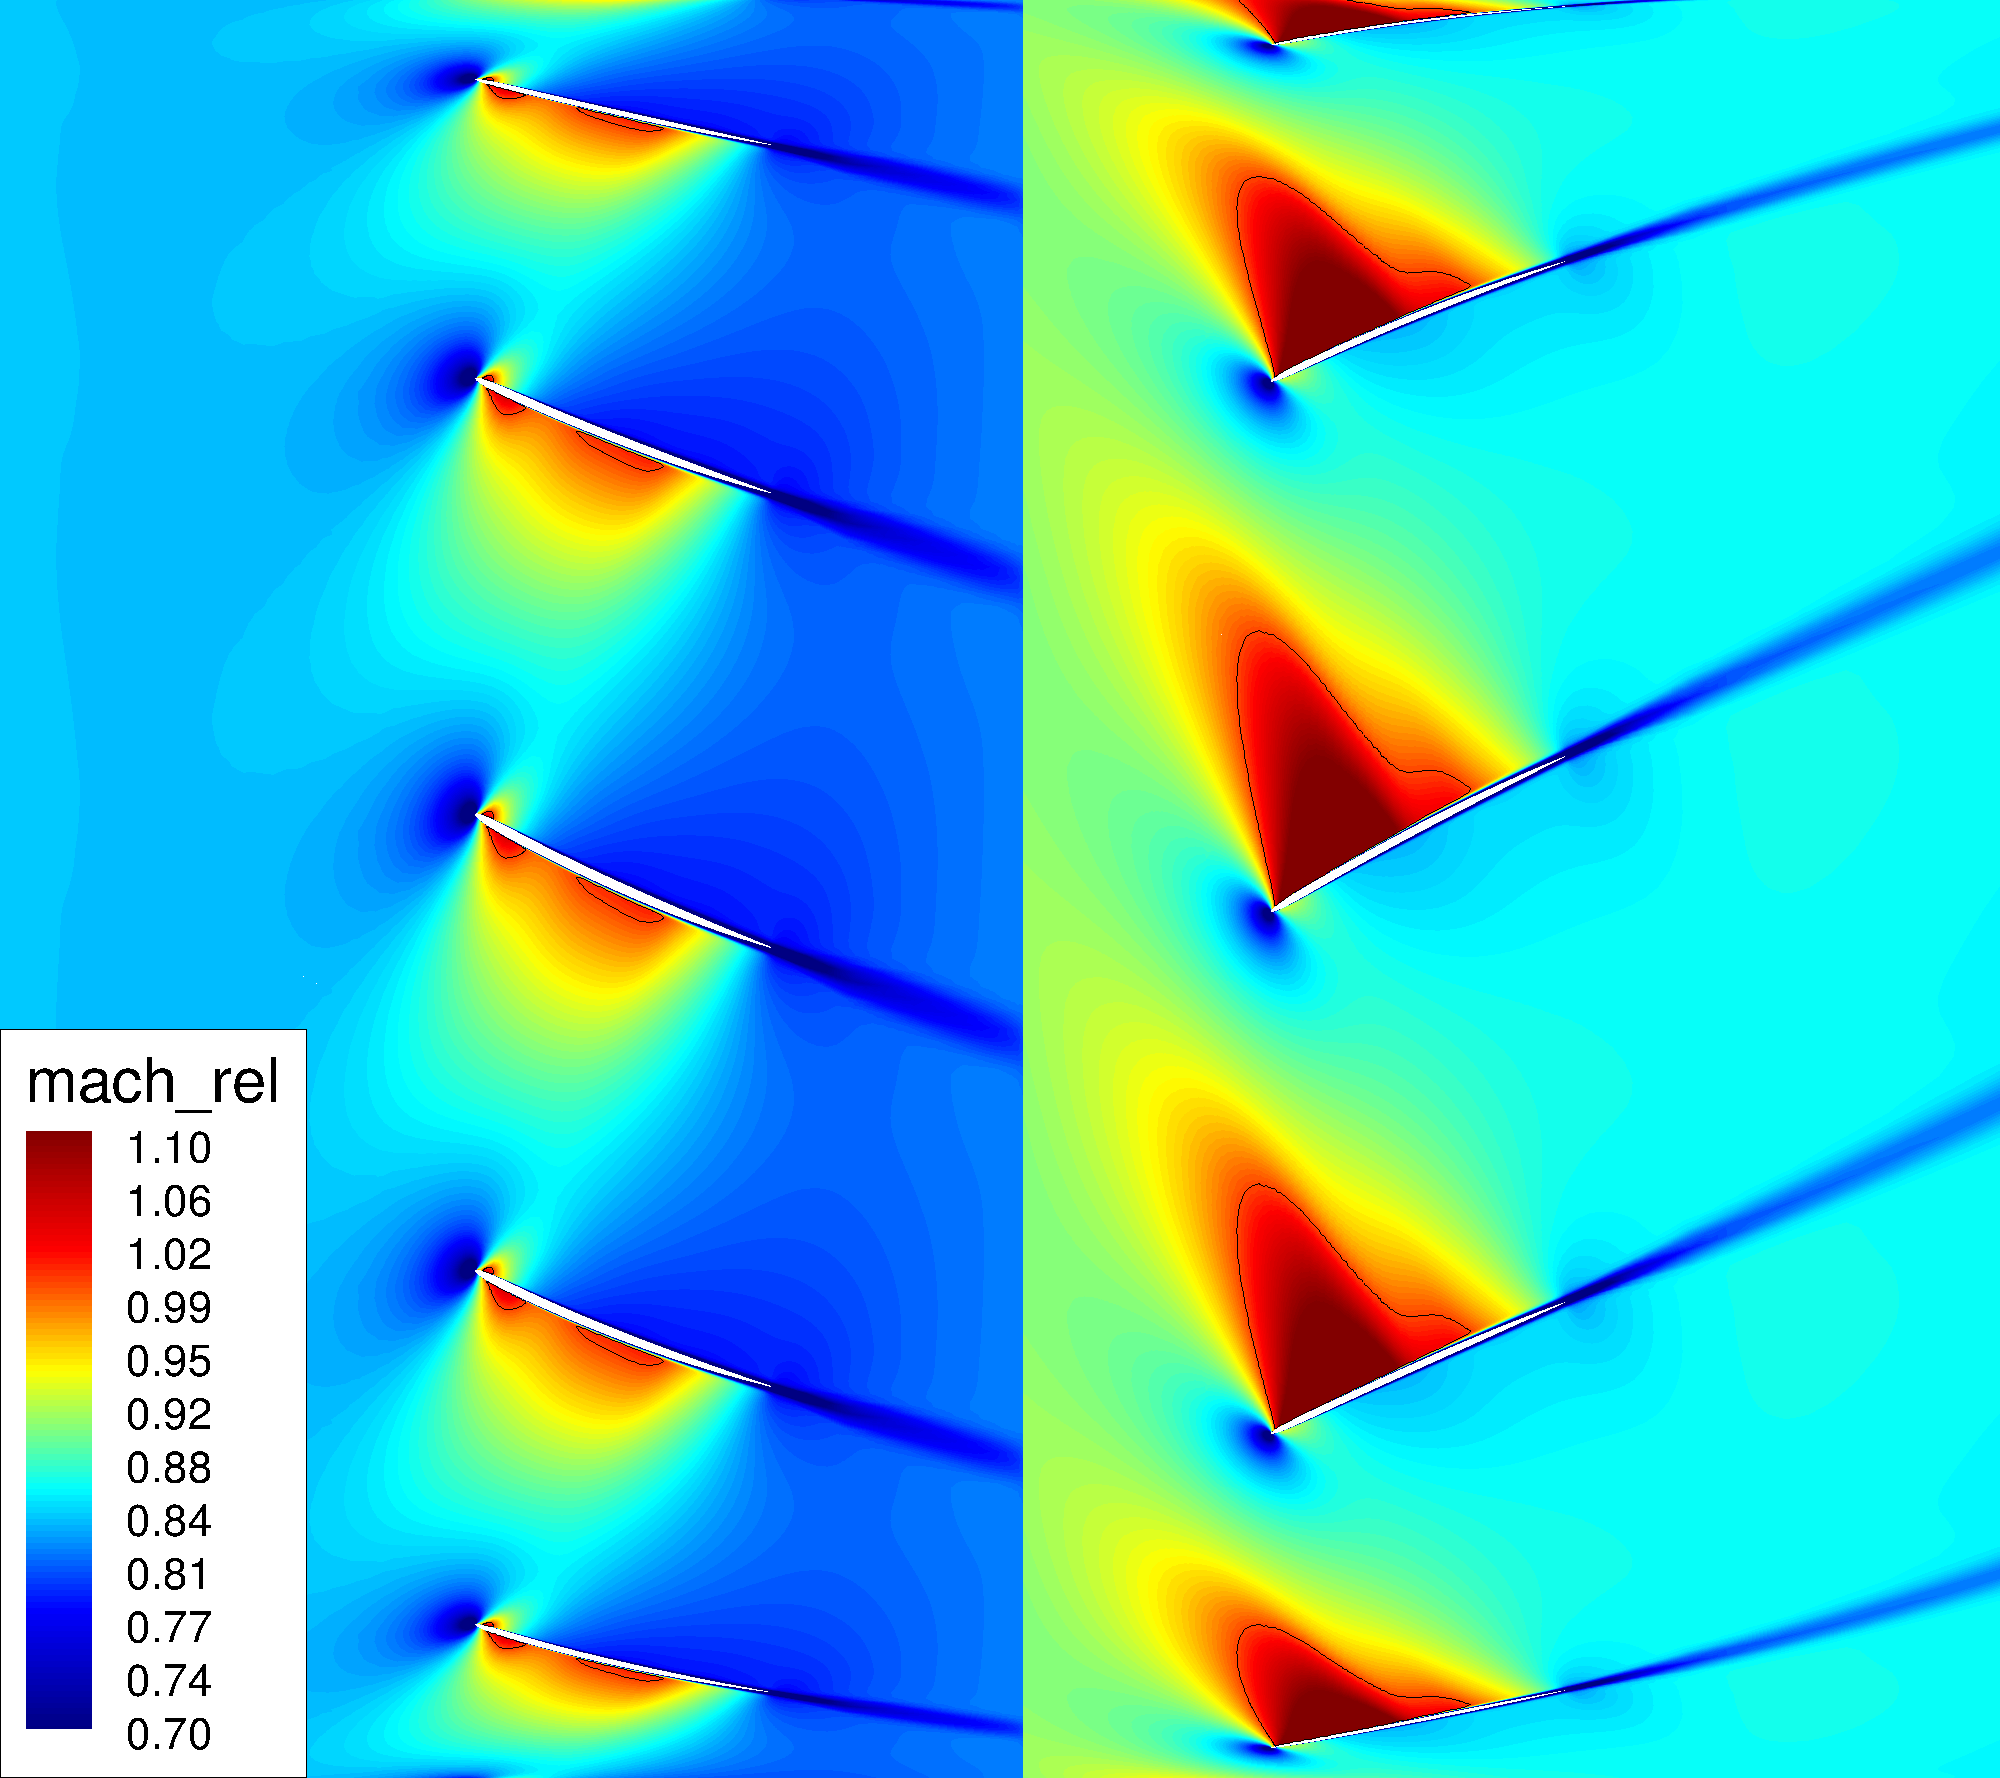
\includegraphics[width=0.28\textwidth]{DREAM_HS_RANS_roe2_sa_slice_r_50_mach_rel.png}\\
   \rotatebox{90}{\qquad\qquad 75~\%} 
   & 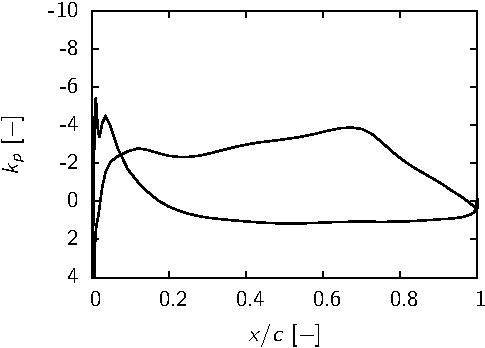
\includegraphics[width=0.28\textwidth]{DREAM_HS_KP_75_FRONT_PPT.pdf}
   & 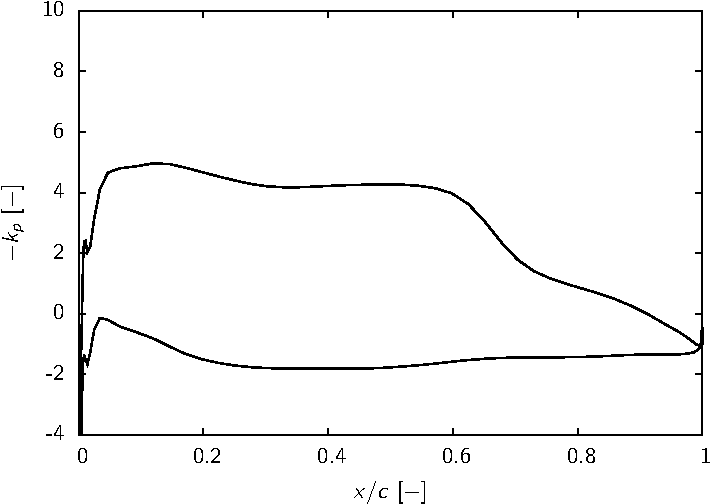
\includegraphics[width=0.28\textwidth]{DREAM_HS_KP_75_REAR_PPT.pdf}
   & 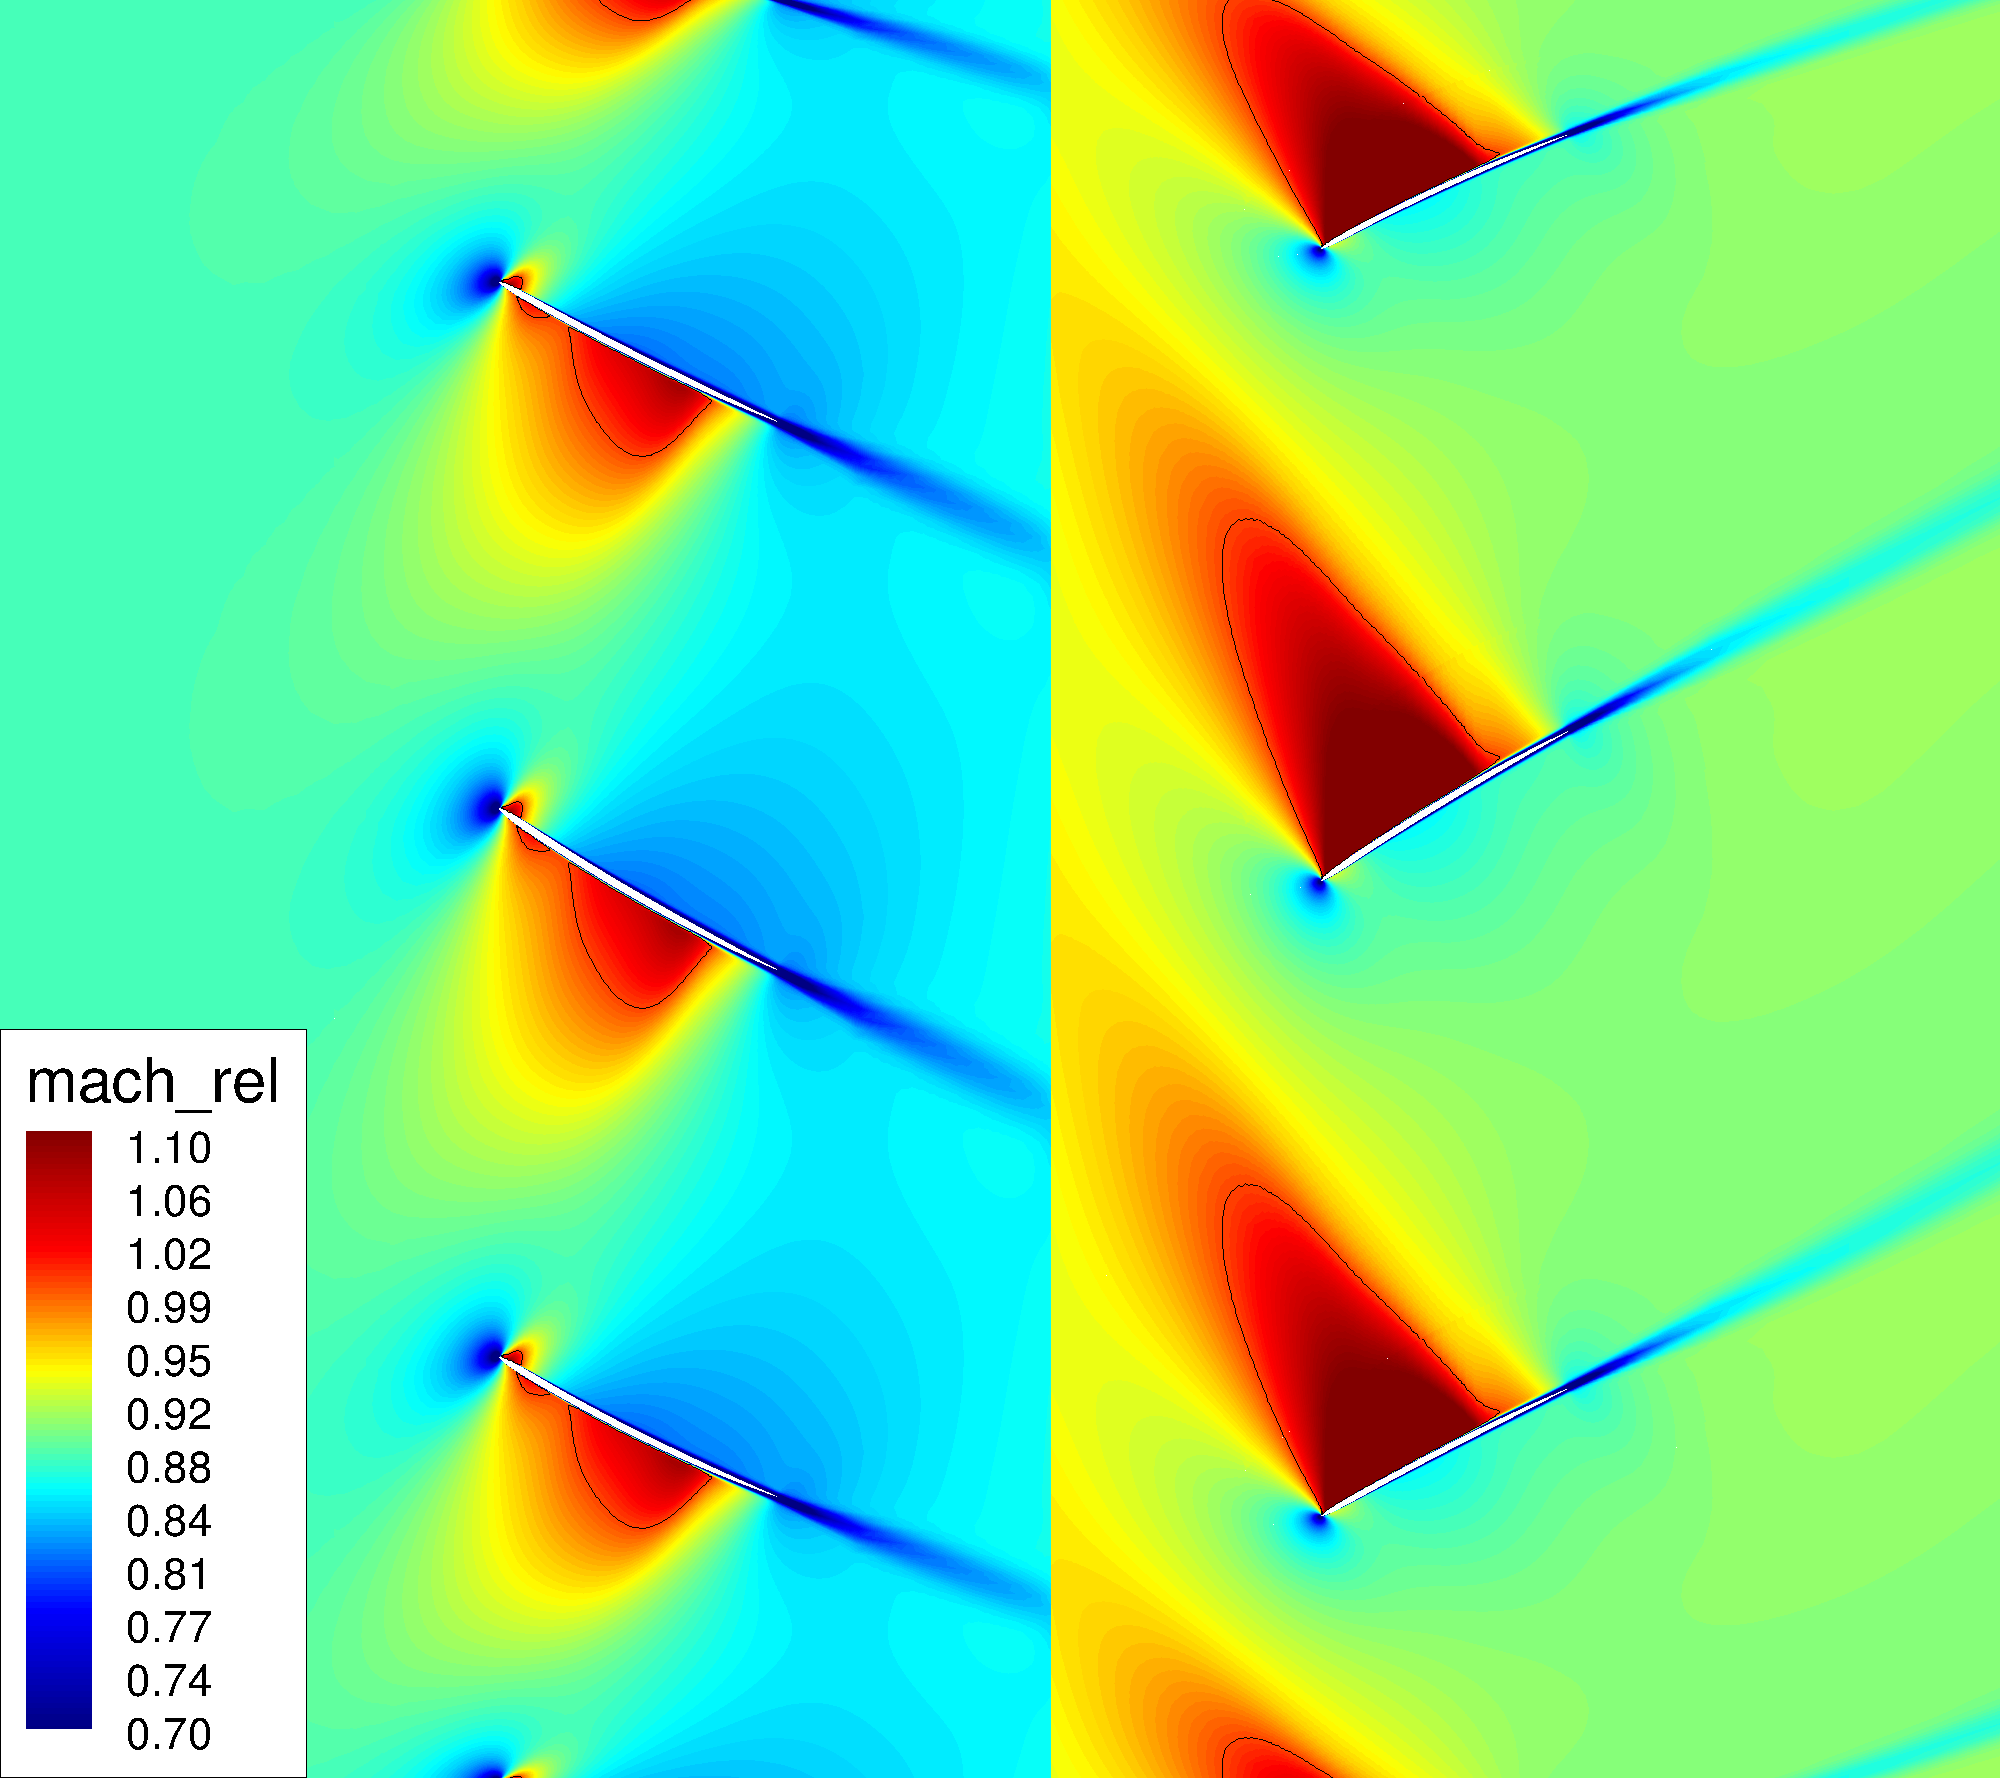
\includegraphics[width=0.28\textwidth]{DREAM_HS_RANS_roe2_sa_slice_r_75_mach_rel.png}\\
   \rotatebox{90}{\qquad\qquad 90~\%} 
   & 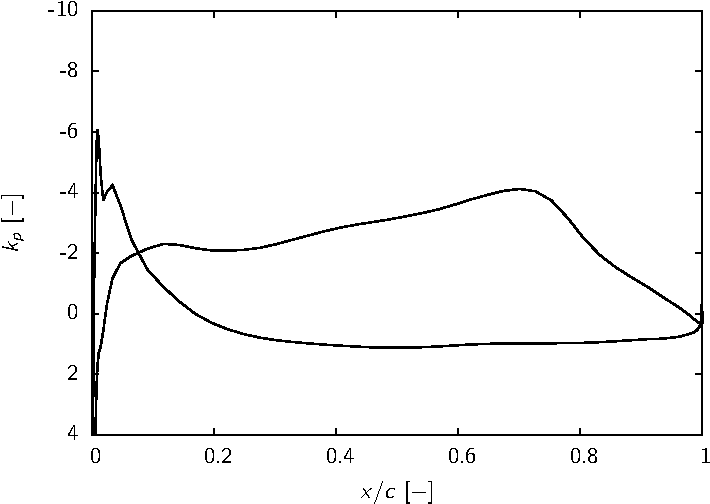
\includegraphics[width=0.28\textwidth]{DREAM_HS_KP_90_FRONT_PPT.pdf}
   & 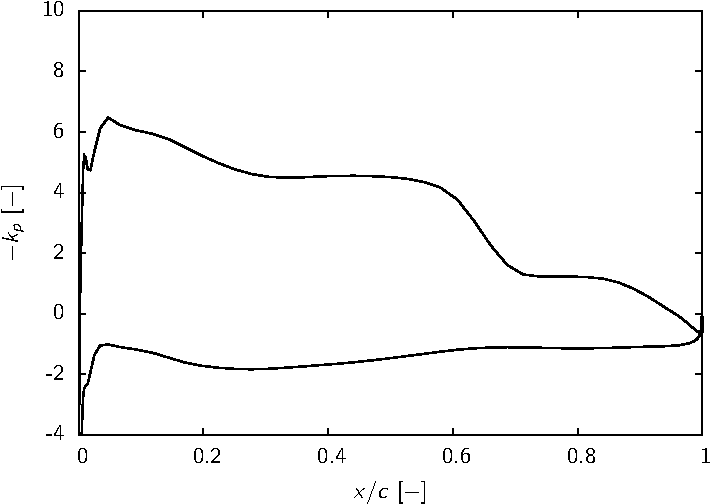
\includegraphics[width=0.28\textwidth]{DREAM_HS_KP_90_REAR_PPT.pdf}
   & 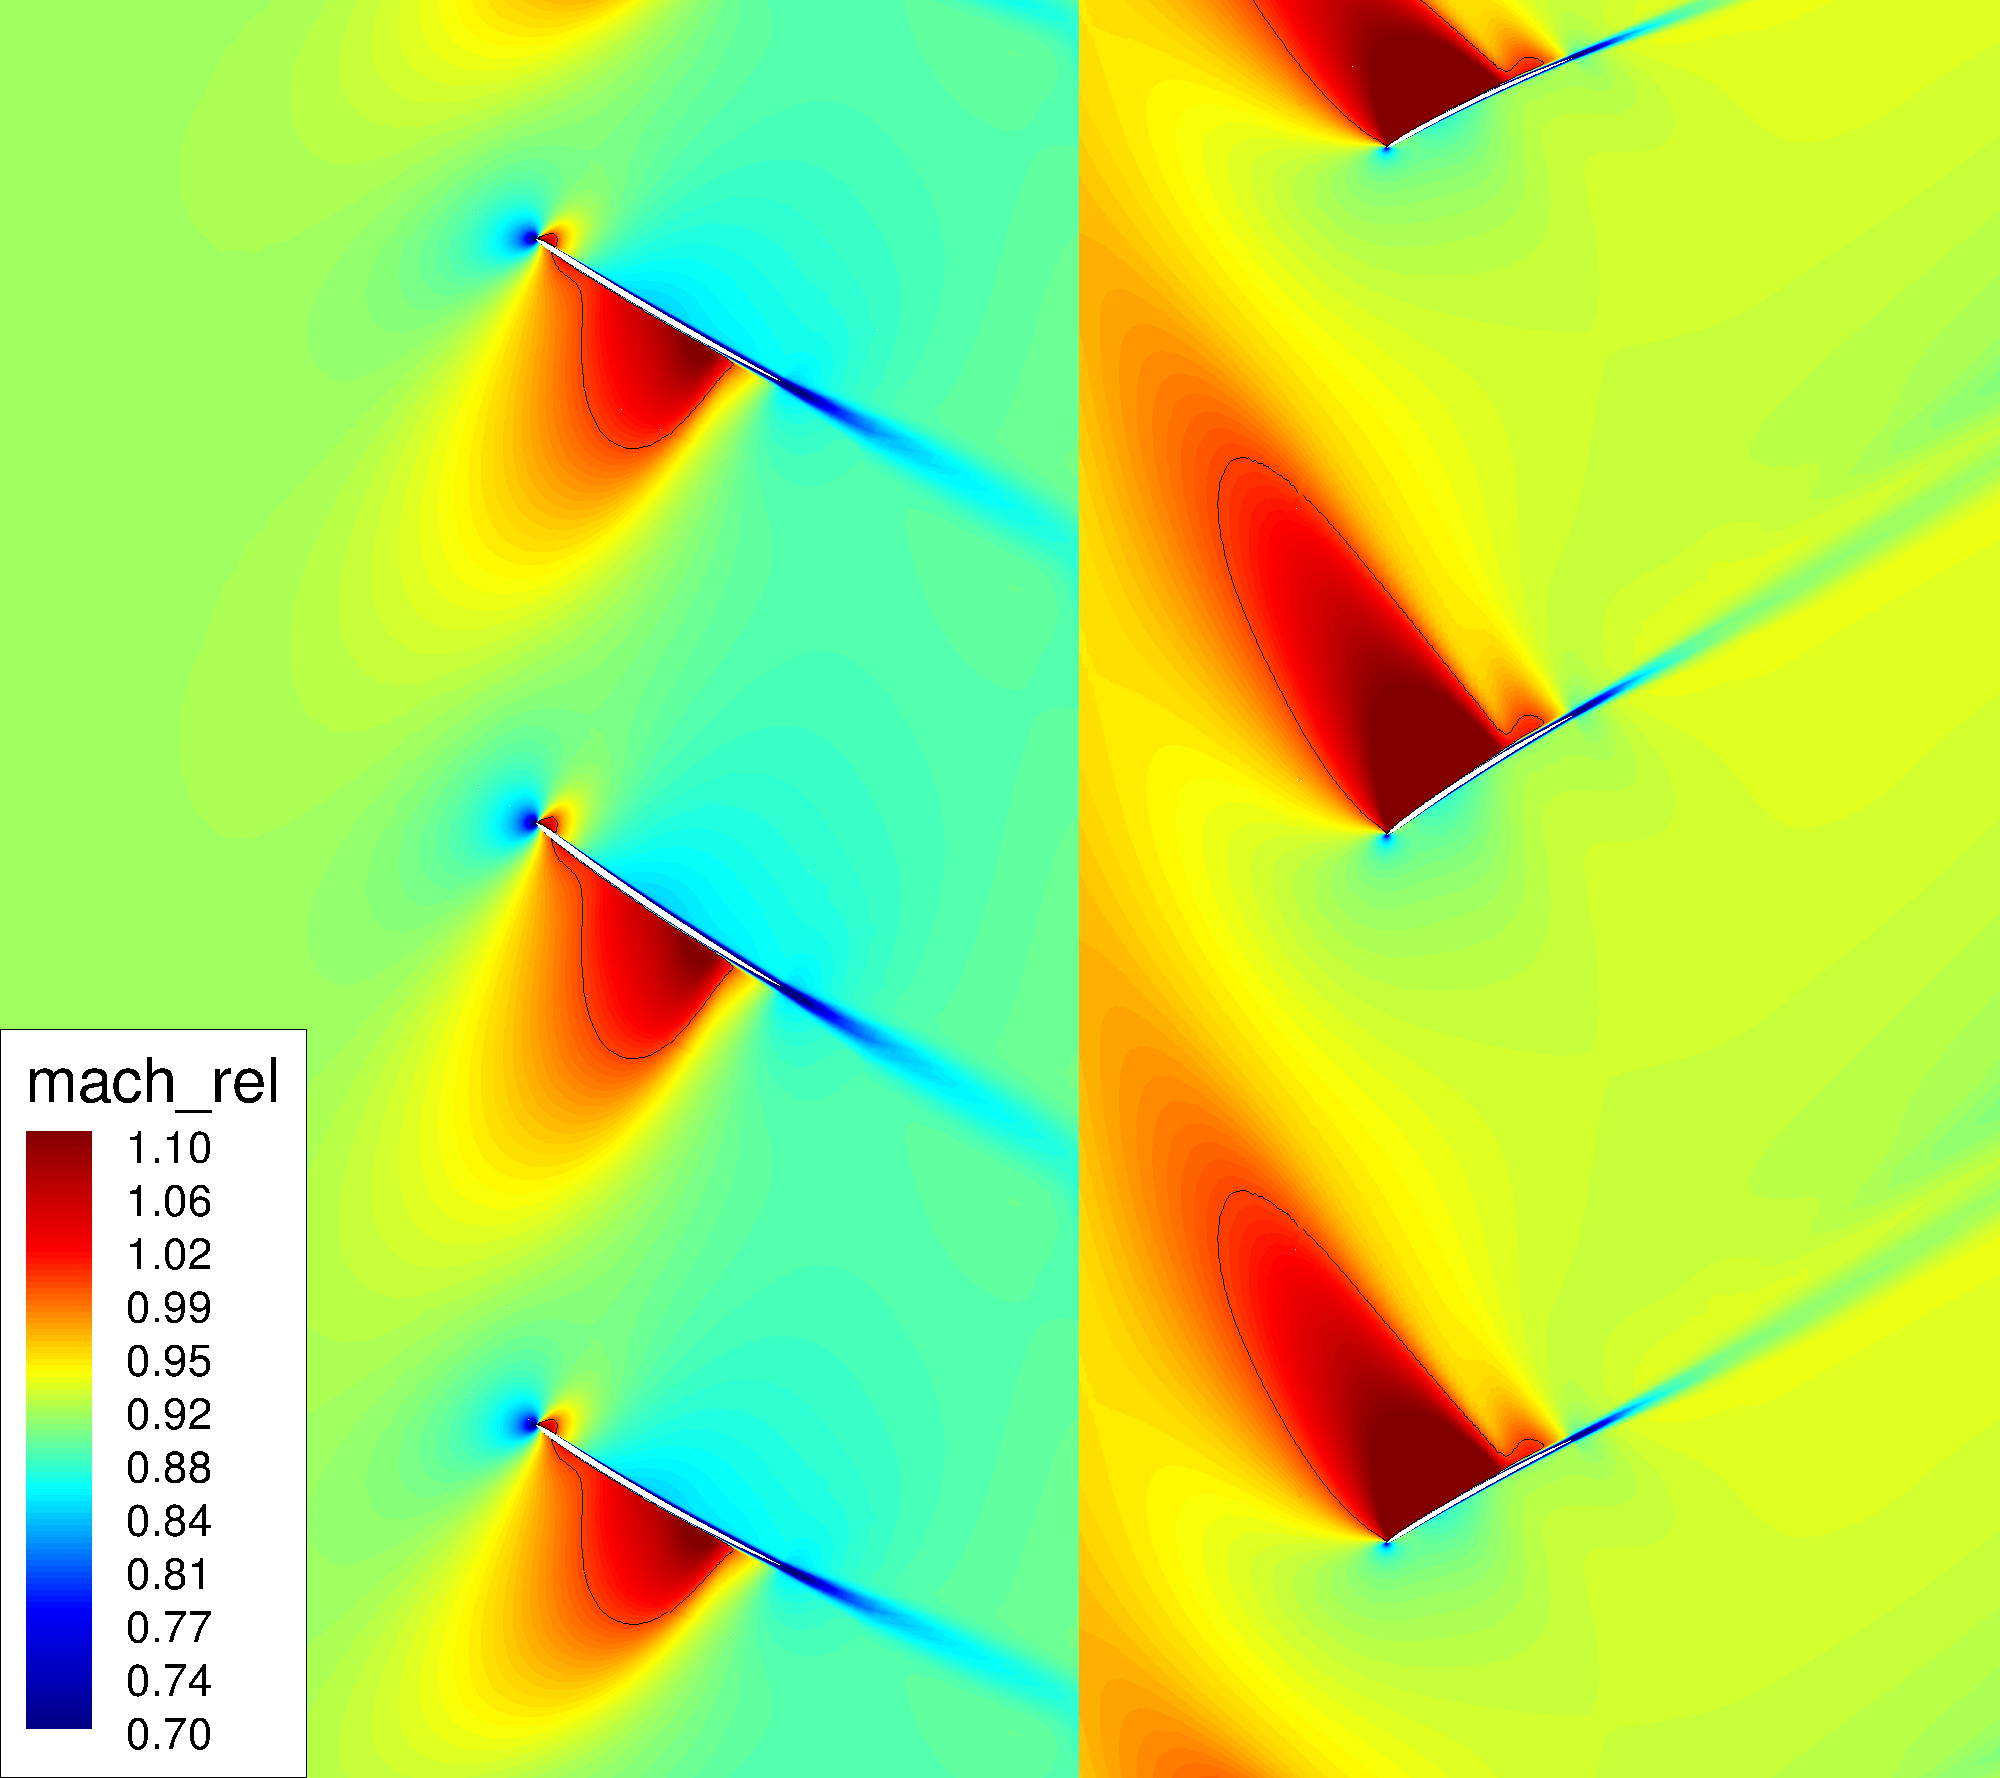
\includegraphics[width=0.28\textwidth]{DREAM_HS_RANS_roe2_sa_slice_r_90_mach_rel.png}\\
   \rotatebox{90}{\qquad\qquad 95~\%} 
   & 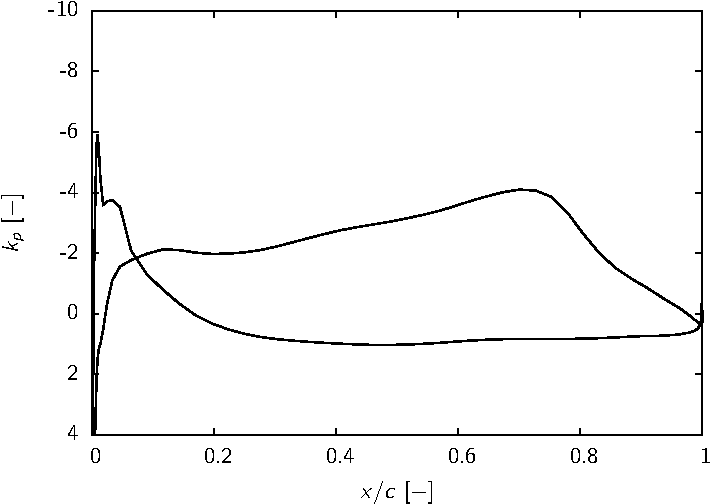
\includegraphics[width=0.28\textwidth]{DREAM_HS_KP_95_FRONT_PPT.pdf}
   & 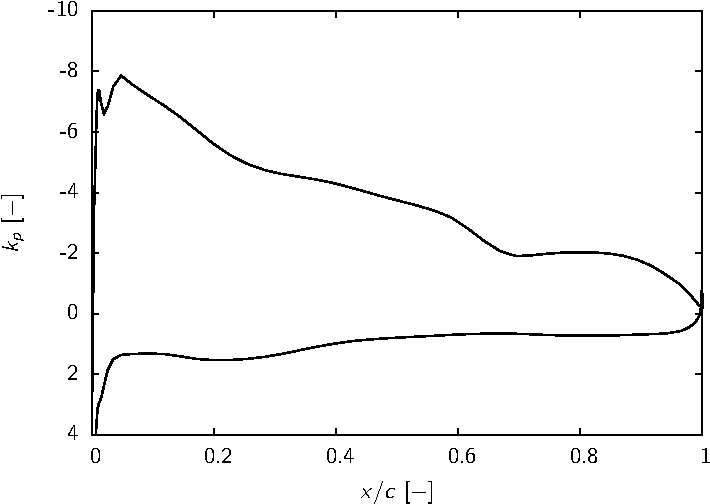
\includegraphics[width=0.28\textwidth]{DREAM_HS_KP_95_REAR_PPT.pdf}
   & 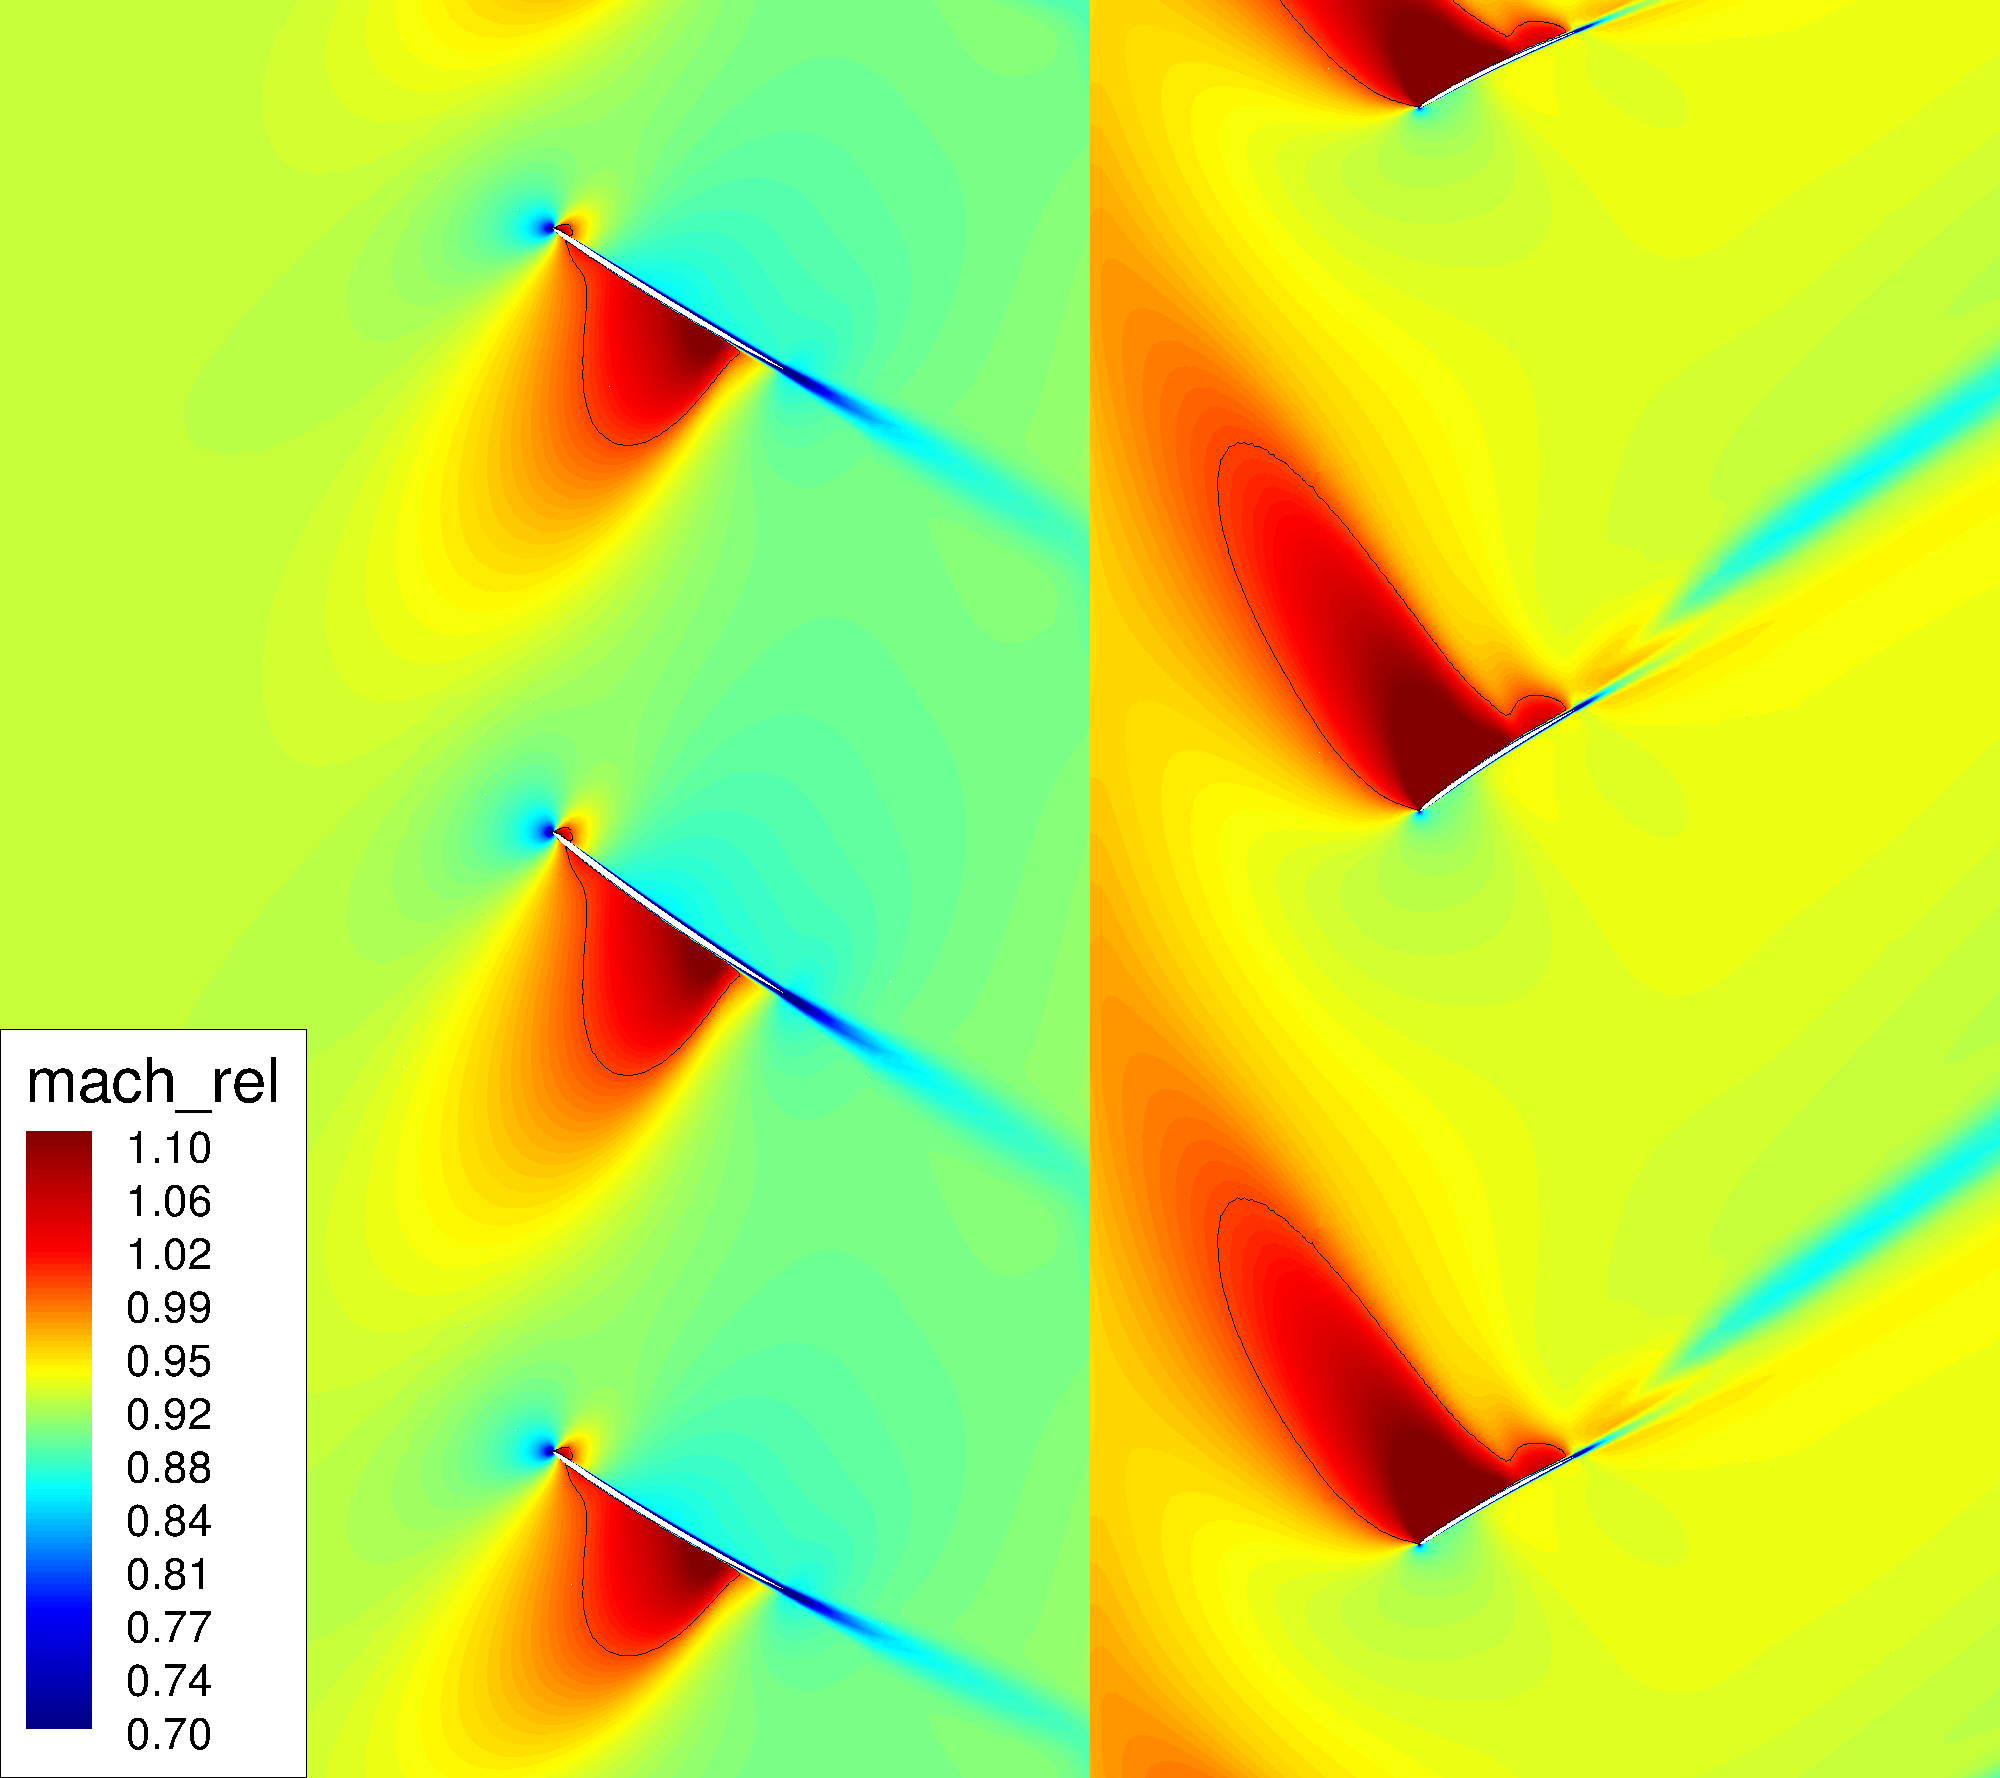
\includegraphics[width=0.28\textwidth]{DREAM_HS_RANS_roe2_sa_slice_r_95_mach_rel.png}  
 \end{tabular}
 \caption{High-speed isolated configuration: pressure coefficient and relative Mach
 number contours at different radial position.}
 \label{fig:dream_HS_mach_kp}
\end{figure}

On the front rotor, for relative span $R / R_f = 25 \%$,
a compression is observed near the leading edge ($x/c \leq 0.2$)
of the suction side. The pressure coefficient is then
almost constant up to the trailing edge. For all
relative spans,
a small negative incidence is indicated by a crossing
in $k_p$ values for all spans of the front rotor,
near the leading edge. This might indicate
that either the incidence of the blades or the rotation speed is
not well adapted for this inflow condition.
The shock that was seen near the leading edge seems to change to a
weak shock wave for higher relative spans ($R / R_f \geq 50 \%$).
On the suction side of the blade, the pressure coefficient $k_p$
increases such that for $R / R_f \geq 75 \%$, a shock is observed
on the suction side of the blade at $x/c \approx 0.7$.

On the rear rotor, the flow field seems to be better adapted to
the inflow conditions. In fact, no negative incidence is seen.
A shock is observed at $x/c \approx 0.5$ for all relative spans
that moves toward the trailing edge as
for $R / R_f = 90 \%$, it is located at $x/c \approx 0.6$.
In fact, as the relative span increases, the relative Mach
number grows which explains the movement of the shock
toward the trailing edge.
For $R / R_f = 95 \%$, no shock is seen but rather a smooth
compression of the flow. This is due to the 
leaving of rear rotor tip vortices that splits the
pressure gradient responsible for the shock.
In fact a low velocity trace seems to indicate
a tip vortex. Globally, the pressure coefficients on the 
rear rotor have a higher integral, explaining
the higher thrust coefficients observed in Sec.~\ref{sub:dream_hs_sim_coeff}.

To investigate the structure of the tip vortices, axial
cuts of entropy made at planes $P3$, $P4$, $P5$ and $P6$
are shown in Figure~\ref{fig:dream_HS_steady_entropy}. One can notice
that the vortices look much thinner compared to the
low-speed inflow condition ones. This is due to the
staggering angle of the blades. In fact, as the inflow 
Mach number is greater, the staggering angle should be
decreased so that an almost constant rotation speed can be kept.
Therefore, projecting the tip vortices on axial cuts will make
the high-speed one thinner. Contrary to the low-speed
inflow condition, the trace of the front rotor tip vortices
seen in plane $P4$ seems to pass above the rear rotor tip
vortices. This was also observed when looking at the radial profiles.
This will be deeply investigated with unsteady simulations
in Sec.~\ref{sec:dream_hs_rigid_results}.
\begin{figure}[htp]
  \centering
  \subfigure[$P3$]{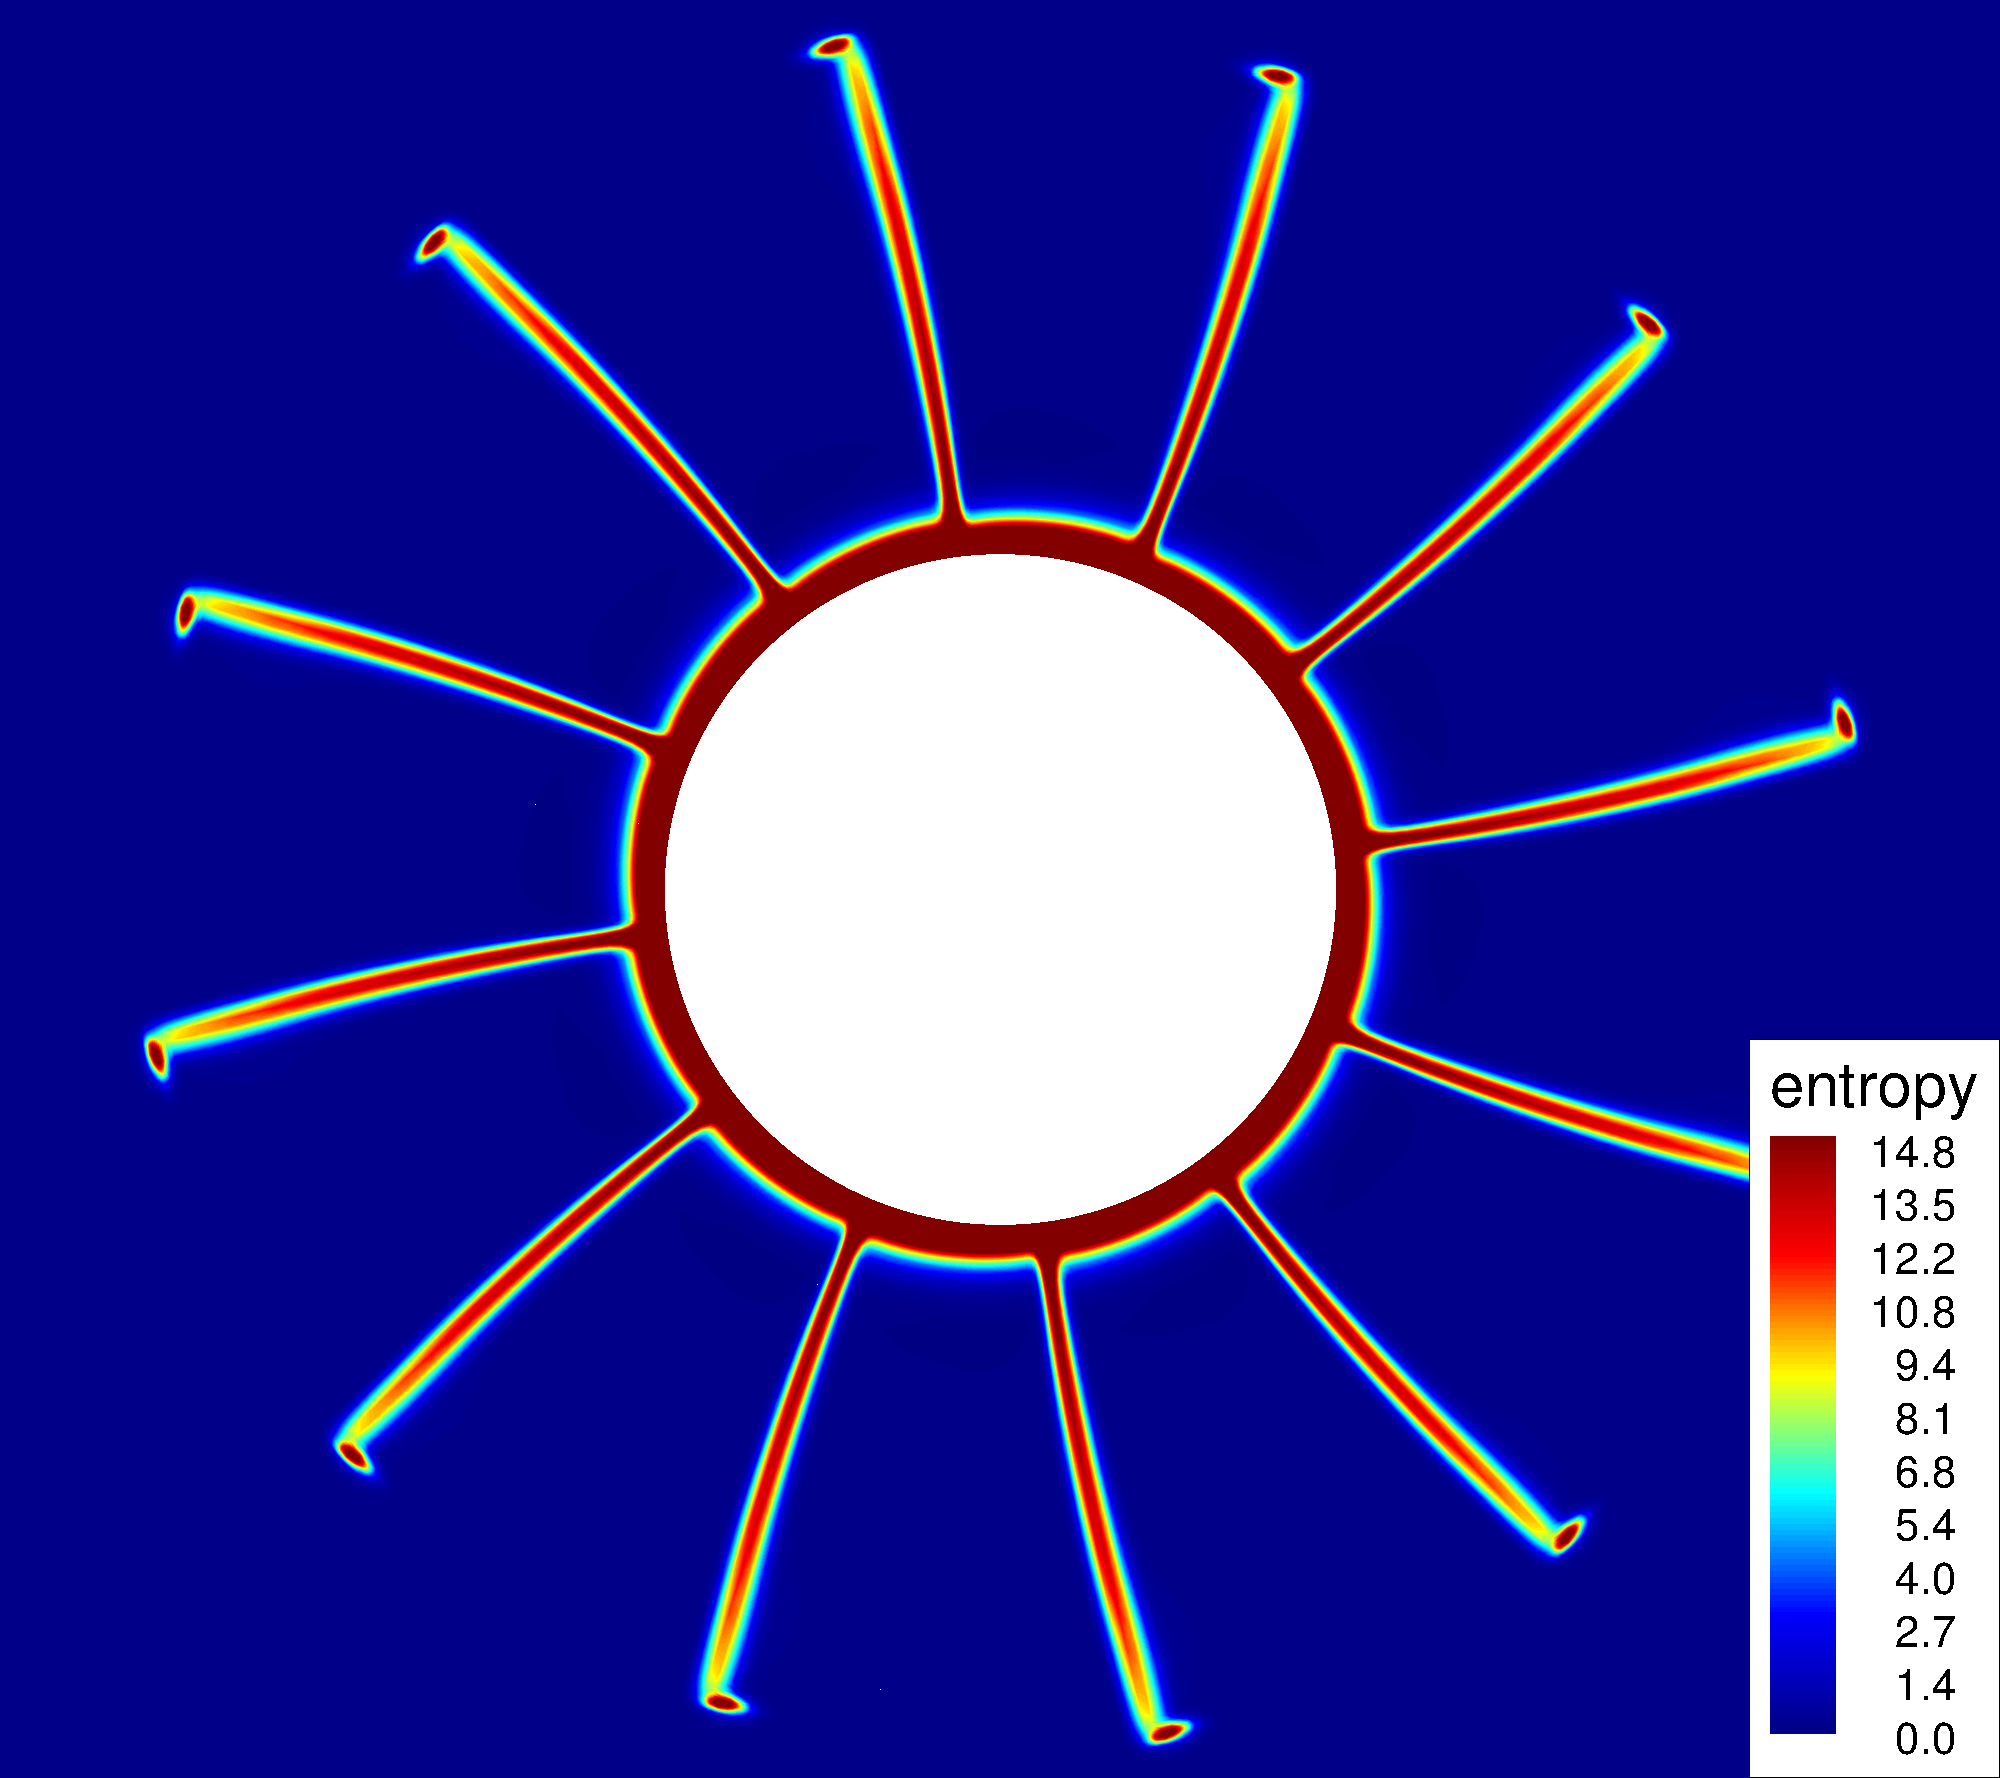
\includegraphics[width=.35\textwidth]{DREAM_HS_RANS_roe2_sa_slice_x_front_1_entropy.png}}
  \subfigure[$P4$]{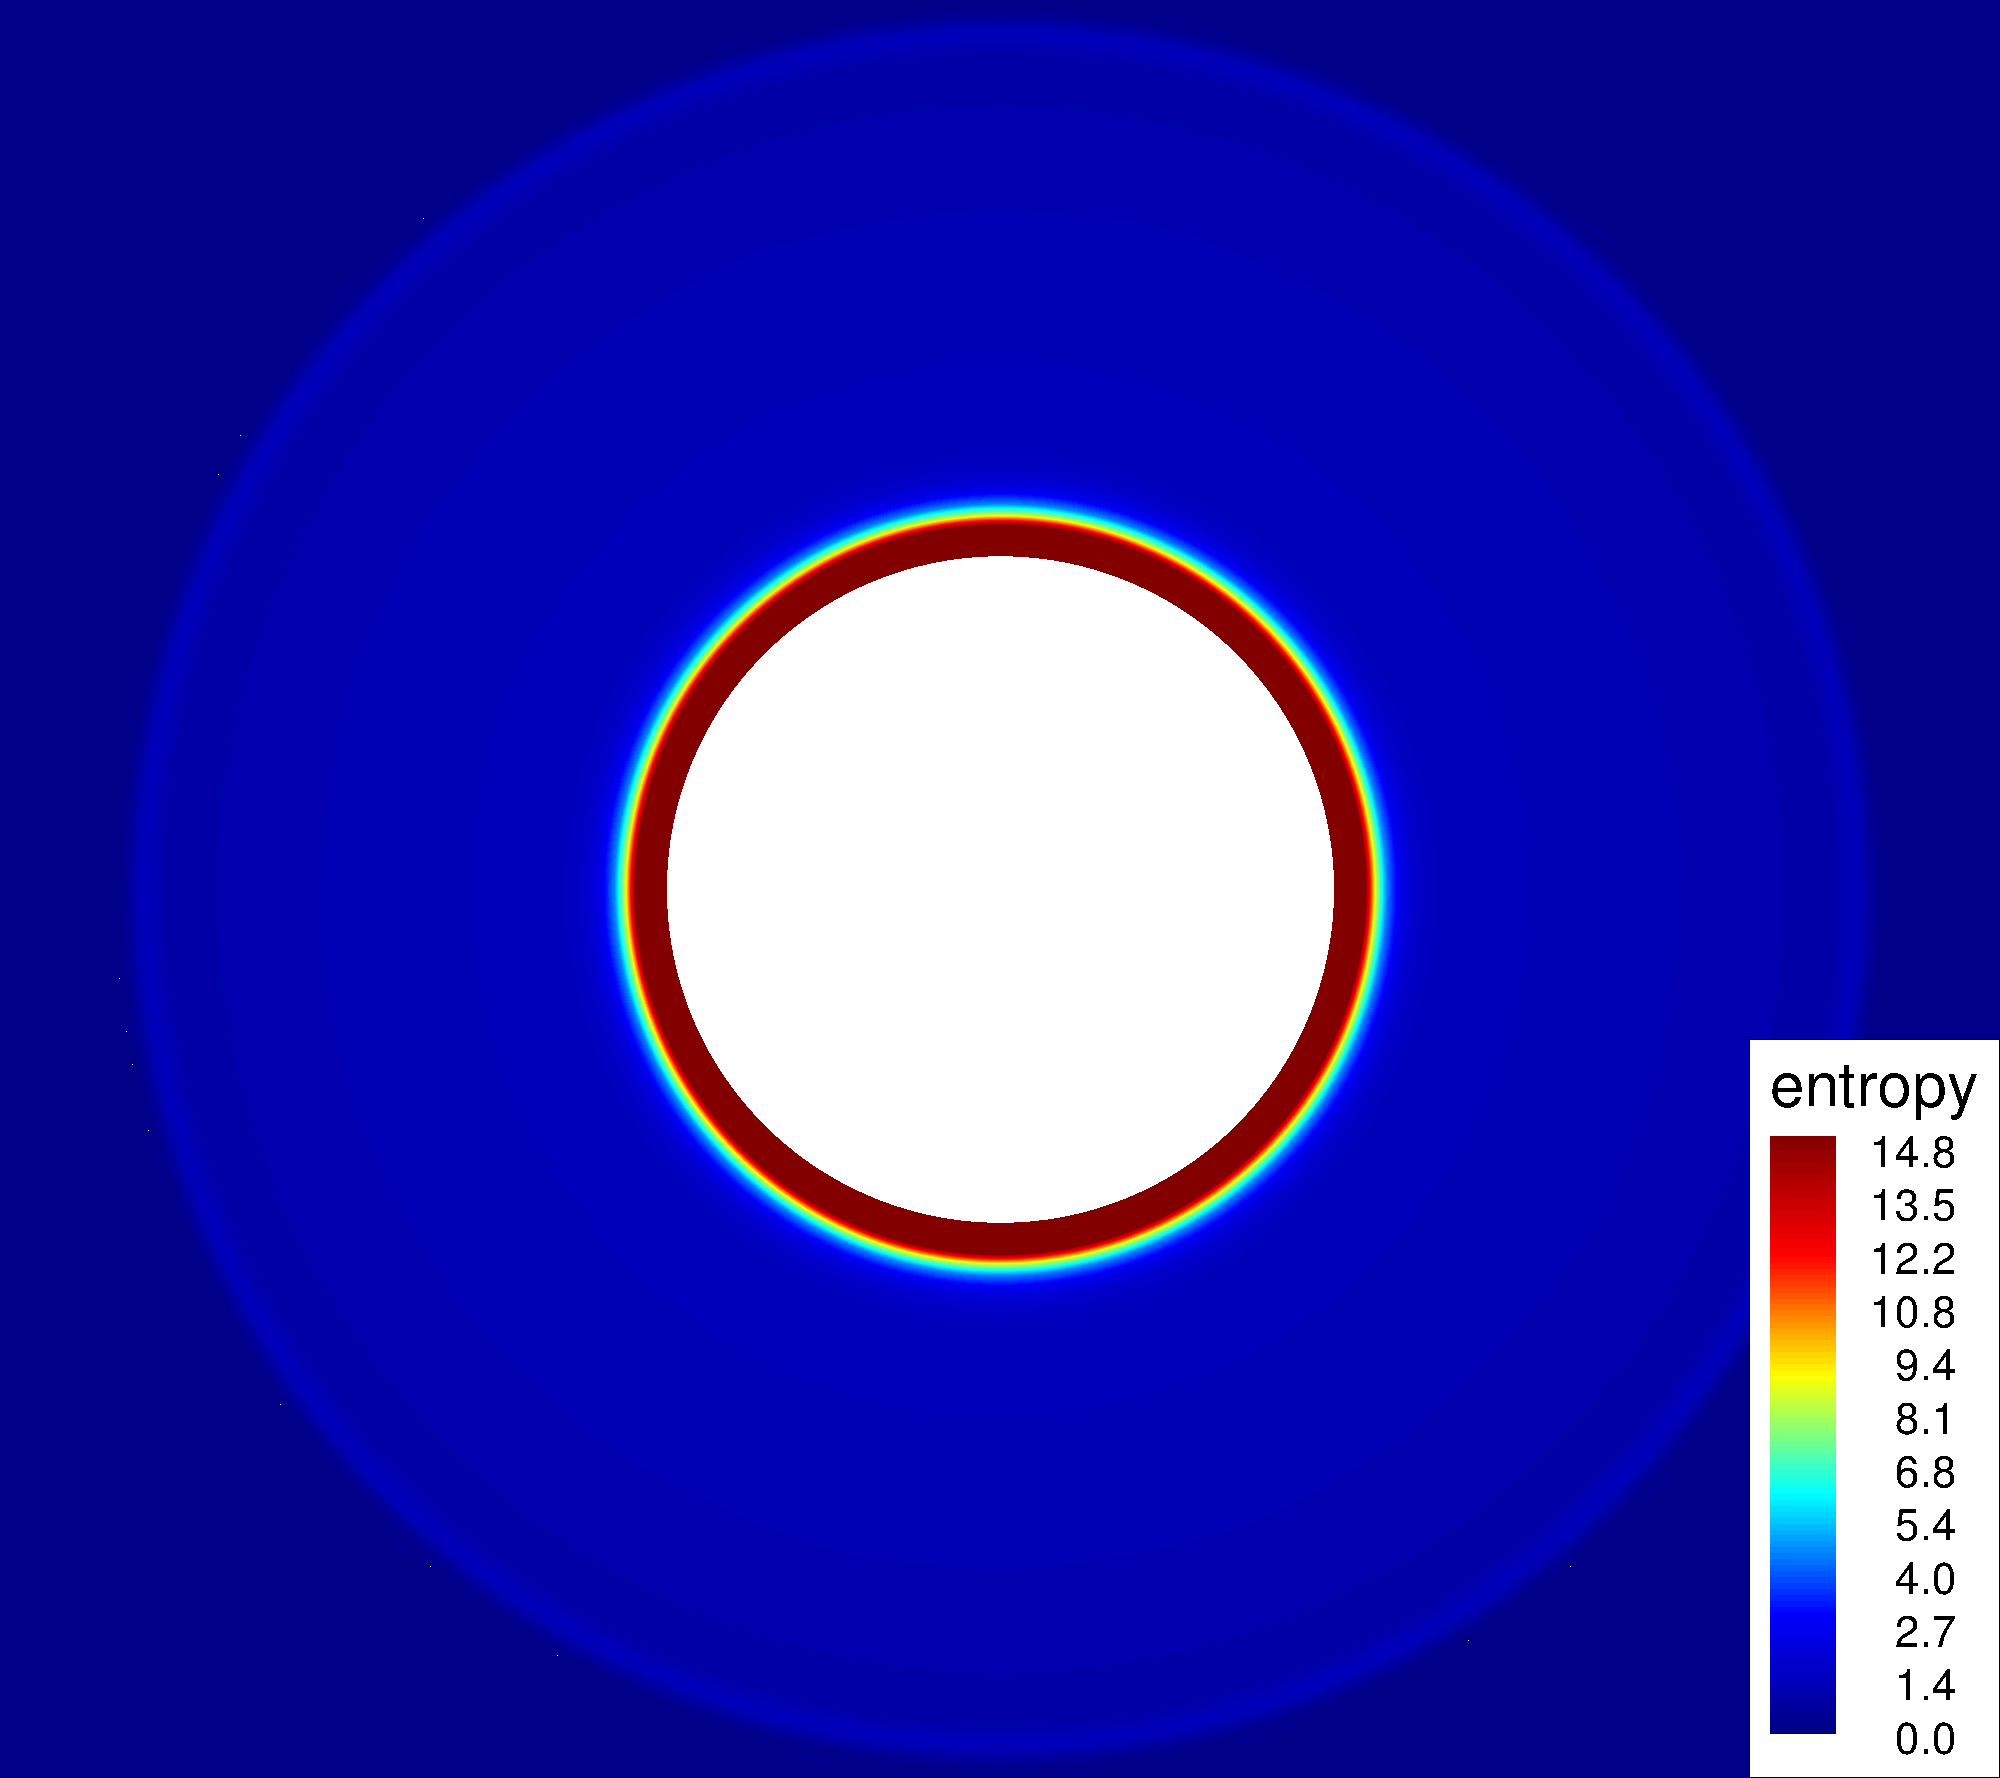
\includegraphics[width=.35\textwidth]{DREAM_HS_RANS_roe2_sa_slice_x_rear_0_entropy.png}}
  \subfigure[$P5$]{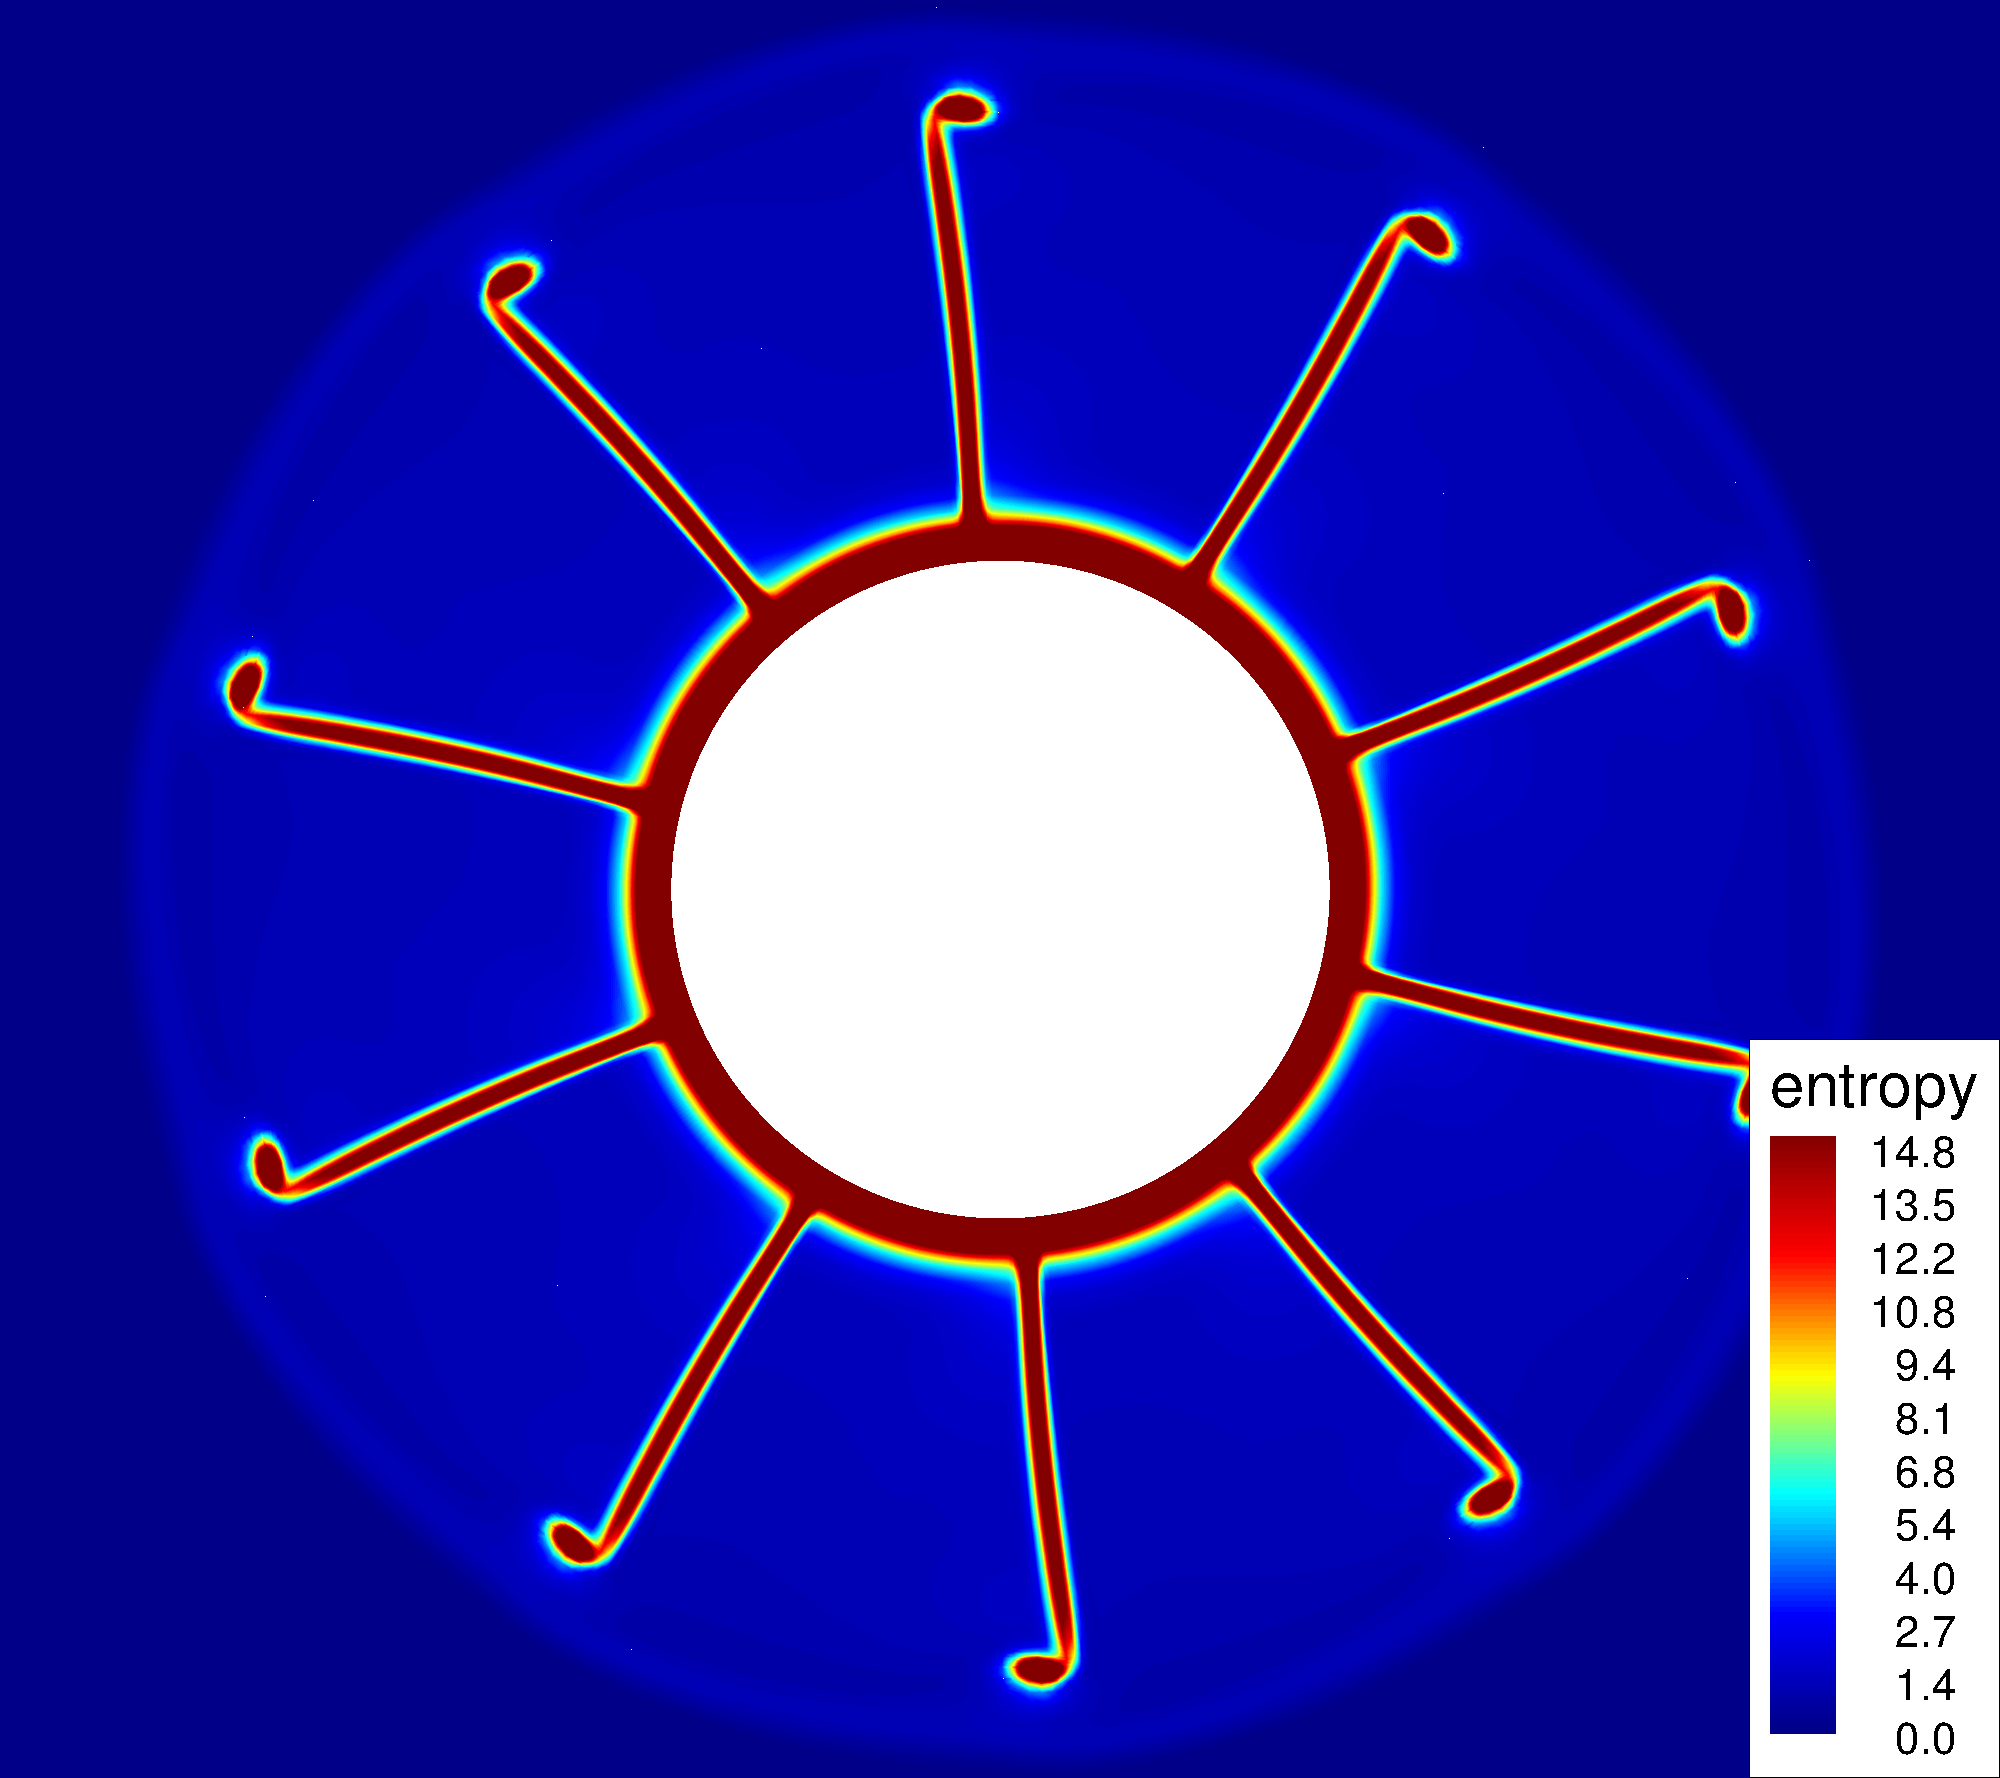
\includegraphics[width=.35\textwidth]{DREAM_HS_RANS_roe2_sa_slice_x_rear_1_entropy.png}}
  \subfigure[$P6$]{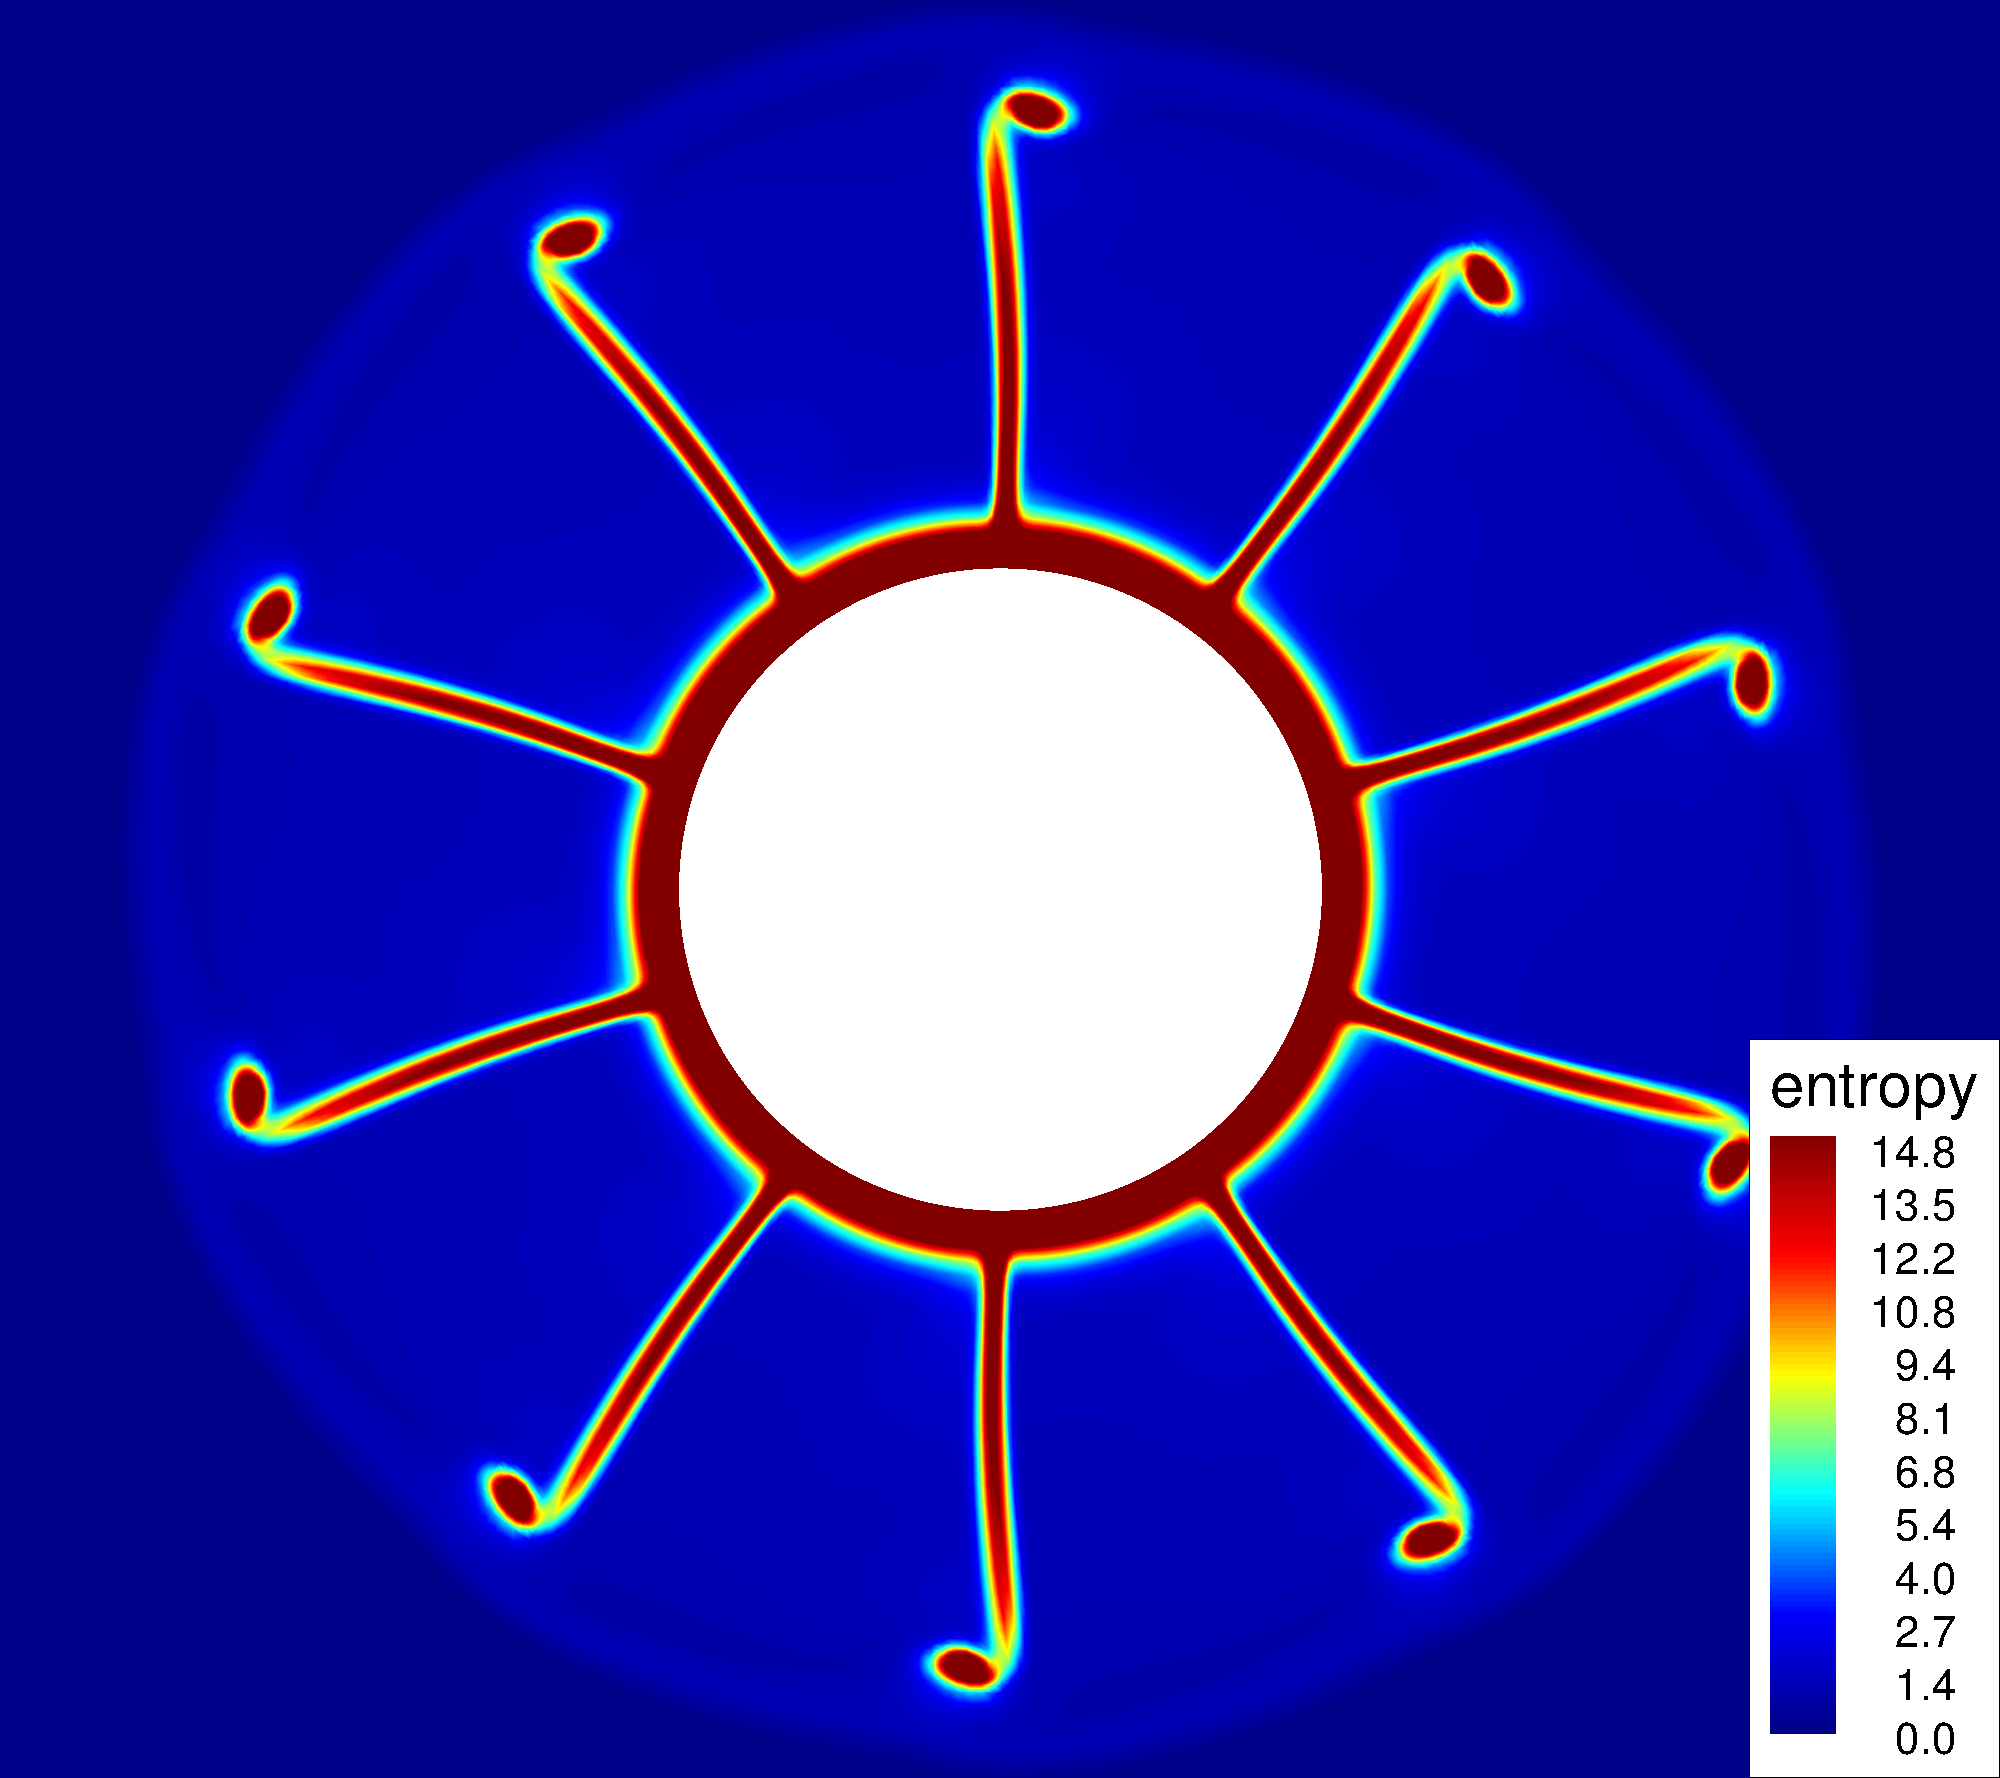
\includegraphics[width=.35\textwidth]{DREAM_HS_RANS_roe2_sa_slice_x_rear_2_entropy.png}}
  \caption{High-speed isolated configuration: axial cut of entropy.}
   \label{fig:dream_HS_steady_entropy}
\end{figure}